\documentclass[twoside]{book}

% Packages required by doxygen
\usepackage{fixltx2e}
\usepackage{calc}
\usepackage{doxygen}
\usepackage[export]{adjustbox} % also loads graphicx
\usepackage{graphicx}
\usepackage[utf8]{inputenc}
\usepackage{makeidx}
\usepackage{multicol}
\usepackage{multirow}
\PassOptionsToPackage{warn}{textcomp}
\usepackage{textcomp}
\usepackage[nointegrals]{wasysym}
\usepackage[table]{xcolor}

% Font selection
\usepackage[T1]{fontenc}
\usepackage[scaled=.90]{helvet}
\usepackage{courier}
\usepackage{amssymb}
\usepackage{sectsty}
\renewcommand{\familydefault}{\sfdefault}
\allsectionsfont{%
  \fontseries{bc}\selectfont%
  \color{darkgray}%
}
\renewcommand{\DoxyLabelFont}{%
  \fontseries{bc}\selectfont%
  \color{darkgray}%
}
\newcommand{\+}{\discretionary{\mbox{\scriptsize$\hookleftarrow$}}{}{}}

% Page & text layout
\usepackage{geometry}
\geometry{%
  a4paper,%
  top=2.5cm,%
  bottom=2.5cm,%
  left=2.5cm,%
  right=2.5cm%
}
\tolerance=750
\hfuzz=15pt
\hbadness=750
\setlength{\emergencystretch}{15pt}
\setlength{\parindent}{0cm}
\setlength{\parskip}{3ex plus 2ex minus 2ex}
\makeatletter
\renewcommand{\paragraph}{%
  \@startsection{paragraph}{4}{0ex}{-1.0ex}{1.0ex}{%
    \normalfont\normalsize\bfseries\SS@parafont%
  }%
}
\renewcommand{\subparagraph}{%
  \@startsection{subparagraph}{5}{0ex}{-1.0ex}{1.0ex}{%
    \normalfont\normalsize\bfseries\SS@subparafont%
  }%
}
\makeatother

% Headers & footers
\usepackage{fancyhdr}
\pagestyle{fancyplain}
\fancyhead[LE]{\fancyplain{}{\bfseries\thepage}}
\fancyhead[CE]{\fancyplain{}{}}
\fancyhead[RE]{\fancyplain{}{\bfseries\leftmark}}
\fancyhead[LO]{\fancyplain{}{\bfseries\rightmark}}
\fancyhead[CO]{\fancyplain{}{}}
\fancyhead[RO]{\fancyplain{}{\bfseries\thepage}}
\fancyfoot[LE]{\fancyplain{}{}}
\fancyfoot[CE]{\fancyplain{}{}}
\fancyfoot[RE]{\fancyplain{}{\bfseries\scriptsize Generated by Doxygen }}
\fancyfoot[LO]{\fancyplain{}{\bfseries\scriptsize Generated by Doxygen }}
\fancyfoot[CO]{\fancyplain{}{}}
\fancyfoot[RO]{\fancyplain{}{}}
\renewcommand{\footrulewidth}{0.4pt}
\renewcommand{\chaptermark}[1]{%
  \markboth{#1}{}%
}
\renewcommand{\sectionmark}[1]{%
  \markright{\thesection\ #1}%
}

% Indices & bibliography
\usepackage{natbib}
\usepackage[titles]{tocloft}
\setcounter{tocdepth}{3}
\setcounter{secnumdepth}{5}
\makeindex

% Hyperlinks (required, but should be loaded last)
\usepackage{ifpdf}
\ifpdf
  \usepackage[pdftex,pagebackref=true]{hyperref}
\else
  \usepackage[ps2pdf,pagebackref=true]{hyperref}
\fi
\hypersetup{%
  colorlinks=true,%
  linkcolor=blue,%
  citecolor=blue,%
  unicode%
}

% Custom commands
\newcommand{\clearemptydoublepage}{%
  \newpage{\pagestyle{empty}\cleardoublepage}%
}

\usepackage{caption}
\captionsetup{labelsep=space,justification=centering,font={bf},singlelinecheck=off,skip=4pt,position=top}

%===== C O N T E N T S =====

\begin{document}

% Titlepage & ToC
\hypersetup{pageanchor=false,
             bookmarksnumbered=true,
             pdfencoding=unicode
            }
\pagenumbering{alph}
\begin{titlepage}
\vspace*{7cm}
\begin{center}%
{\Large My Project }\\
\vspace*{1cm}
{\large Generated by Doxygen 1.8.13}\\
\end{center}
\end{titlepage}
\clearemptydoublepage
\pagenumbering{roman}
\tableofcontents
\clearemptydoublepage
\pagenumbering{arabic}
\hypersetup{pageanchor=true}

%--- Begin generated contents ---
\chapter{Hierarchical Index}
\section{Class Hierarchy}
This inheritance list is sorted roughly, but not completely, alphabetically\+:\begin{DoxyCompactList}
\item \contentsline{section}{Dicom\+Dictionary\+Interface}{\pageref{class_dicom_dictionary_interface}}{}
\item \contentsline{section}{Dicom\+Parameters\+Reader}{\pageref{class_dicom_parameters_reader}}{}
\item \contentsline{section}{Dicom\+Series\+Writer}{\pageref{class_dicom_series_writer}}{}
\item \contentsline{section}{Image\+Reader}{\pageref{class_image_reader}}{}
\item Q\+Dialog\begin{DoxyCompactList}
\item \contentsline{section}{Dicom\+Attributes\+Dialog}{\pageref{class_dicom_attributes_dialog}}{}
\end{DoxyCompactList}
\item Q\+Main\+Window\begin{DoxyCompactList}
\item \contentsline{section}{Main\+Window}{\pageref{class_main_window}}{}
\end{DoxyCompactList}
\item Q\+Settings\begin{DoxyCompactList}
\item \contentsline{section}{Settings}{\pageref{class_settings}}{}
\end{DoxyCompactList}
\item \contentsline{section}{Series\+Converter}{\pageref{class_series_converter}}{}
\item \contentsline{section}{Series\+Info}{\pageref{class_series_info}}{}
\end{DoxyCompactList}

\chapter{Class Index}
\section{Class List}
Here are the classes, structs, unions and interfaces with brief descriptions\+:\begin{DoxyCompactList}
\item\contentsline{section}{\hyperlink{class_dicom_attributes_dialog}{Dicom\+Attributes\+Dialog} }{\pageref{class_dicom_attributes_dialog}}{}
\item\contentsline{section}{\hyperlink{class_dicom_dictionary_interface}{Dicom\+Dictionary\+Interface} \\*The \hyperlink{class_dicom_dictionary_interface}{Dicom\+Dictionary\+Interface} class This class provides a convenient to get and set data in an instance of itk\+::\+Meta\+Data\+Dictionary\+Array }{\pageref{class_dicom_dictionary_interface}}{}
\item\contentsline{section}{\hyperlink{class_dicom_parameters_reader}{Dicom\+Parameters\+Reader} \\*Class to read a dicom series and extract parameters from its dictionary, placing them into the global \hyperlink{class_series_info}{Series\+Info} instance }{\pageref{class_dicom_parameters_reader}}{}
\item\contentsline{section}{\hyperlink{class_dicom_series_writer}{Dicom\+Series\+Writer} \\*Class to write a D\+I\+C\+OM series }{\pageref{class_dicom_series_writer}}{}
\item\contentsline{section}{\hyperlink{class_image_reader}{Image\+Reader} \\*Reads an image on disk, creating a std\+::vector of slices }{\pageref{class_image_reader}}{}
\item\contentsline{section}{\hyperlink{class_main_window}{Main\+Window} }{\pageref{class_main_window}}{}
\item\contentsline{section}{\hyperlink{class_series_converter}{Series\+Converter} \\*The \hyperlink{class_series_converter}{Series\+Converter} class }{\pageref{class_series_converter}}{}
\item\contentsline{section}{\hyperlink{class_series_info}{Series\+Info} \\*The \hyperlink{class_series_info}{Series\+Info} class This class contains all of the D\+I\+C\+OM and other information needed to do the conversions }{\pageref{class_series_info}}{}
\item\contentsline{section}{\hyperlink{class_settings}{Settings} \\*The \hyperlink{class_settings}{Settings} class Class which saves and restores settings between executions }{\pageref{class_settings}}{}
\end{DoxyCompactList}

\chapter{Class Documentation}
\hypertarget{class_dicom_attributes_dialog}{}\section{Dicom\+Attributes\+Dialog Class Reference}
\label{class_dicom_attributes_dialog}\index{Dicom\+Attributes\+Dialog@{Dicom\+Attributes\+Dialog}}
Inheritance diagram for Dicom\+Attributes\+Dialog\+:\begin{figure}[H]
\begin{center}
\leavevmode
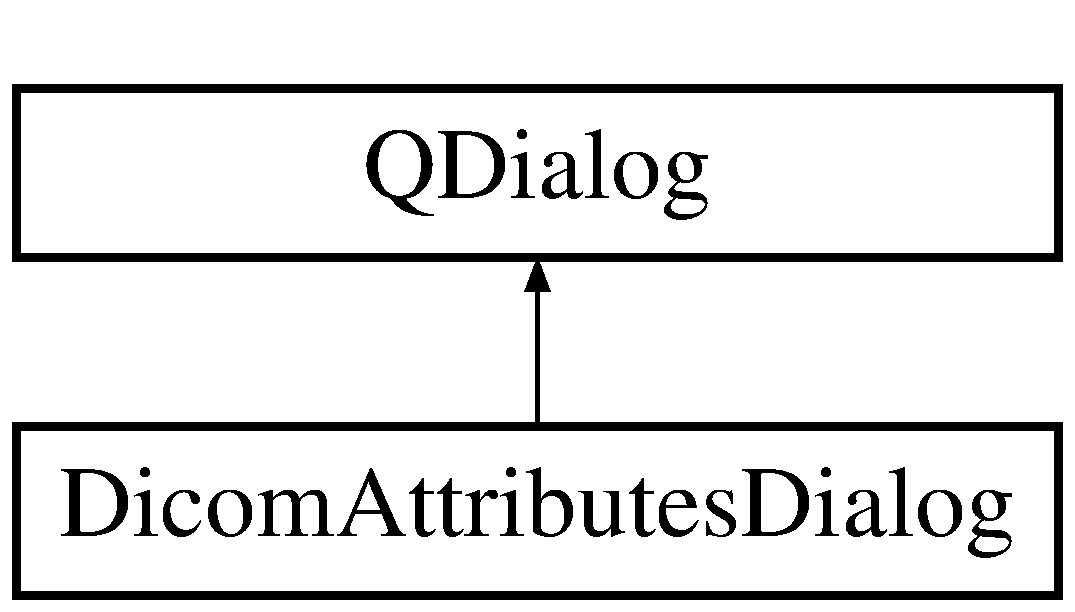
\includegraphics[height=2.000000cm]{class_dicom_attributes_dialog}
\end{center}
\end{figure}
\subsection*{Public Member Functions}
\begin{DoxyCompactItemize}
\item 
\mbox{\Hypertarget{class_dicom_attributes_dialog_a9d229081ef7e02c39d70b9550ca67871}\label{class_dicom_attributes_dialog_a9d229081ef7e02c39d70b9550ca67871}} 
{\bfseries Dicom\+Attributes\+Dialog} (Q\+Widget $\ast$parent=0)
\item 
\mbox{\Hypertarget{class_dicom_attributes_dialog_a2dec90cf3801a1f56cb1e9f3b4af0d6d}\label{class_dicom_attributes_dialog_a2dec90cf3801a1f56cb1e9f3b4af0d6d}} 
void {\bfseries load\+Data} ()
\item 
\mbox{\Hypertarget{class_dicom_attributes_dialog_ad5754486b8b8fea295e8a616363fb24e}\label{class_dicom_attributes_dialog_ad5754486b8b8fea295e8a616363fb24e}} 
void {\bfseries store\+Data} ()
\end{DoxyCompactItemize}


The documentation for this class was generated from the following files\+:\begin{DoxyCompactItemize}
\item 
dicomattributesdialog.\+h\item 
dicomattributesdialog.\+cpp\end{DoxyCompactItemize}

\hypertarget{class_dicom_dictionary_interface}{}\section{Dicom\+Dictionary\+Interface Class Reference}
\label{class_dicom_dictionary_interface}\index{Dicom\+Dictionary\+Interface@{Dicom\+Dictionary\+Interface}}


The \hyperlink{class_dicom_dictionary_interface}{Dicom\+Dictionary\+Interface} class This class provides a convenient to get and set data in an instance of itk\+::\+Meta\+Data\+Dictionary\+Array.  




{\ttfamily \#include $<$dicomdictionaryinterface.\+h$>$}

\subsection*{Public Types}
\begin{DoxyCompactItemize}
\item 
\mbox{\Hypertarget{class_dicom_dictionary_interface_a9fa034992ec9eadd94f1258c2b4458e4}\label{class_dicom_dictionary_interface_a9fa034992ec9eadd94f1258c2b4458e4}} 
typedef std\+::vector$<$ itk\+::\+Meta\+Data\+Dictionary $\ast$ $>$ {\bfseries Dictionary\+Array\+Type}
\item 
typedef Dictionary\+Array\+Type\+::size\+\_\+type \hyperlink{class_dicom_dictionary_interface_a4fde43e0647ab57f29eb2c59c3d051ca}{Size\+Type}
\begin{DoxyCompactList}\small\item\em This typedef is created merely to prevent compiler warnings. \end{DoxyCompactList}\end{DoxyCompactItemize}
\subsection*{Public Member Functions}
\begin{DoxyCompactItemize}
\item 
\hyperlink{class_dicom_dictionary_interface_a8c97276448308399415acccb9608af44}{Dicom\+Dictionary\+Interface} (Dictionary\+Array\+Type dictionary\+Array)
\begin{DoxyCompactList}\small\item\em Constructor with dictionary array. \end{DoxyCompactList}\item 
Q\+String \hyperlink{class_dicom_dictionary_interface_a1e774258d452b2054b90db885eb7915e}{patients\+Name} ()
\begin{DoxyCompactList}\small\item\em Get the value of Patient\textquotesingle{}s Name, \char`\"{}0010$\vert$0010\char`\"{}. \end{DoxyCompactList}\item 
bool \hyperlink{class_dicom_dictionary_interface_a7f951011d920b735e5945b4641790379}{set\+Patients\+Name} (Q\+String \hyperlink{class_dicom_dictionary_interface_a1e774258d452b2054b90db885eb7915e}{patients\+Name})
\begin{DoxyCompactList}\small\item\em Set the value of Patient\textquotesingle{}s Name, \char`\"{}0010$\vert$0010\char`\"{}. \end{DoxyCompactList}\item 
Q\+String \hyperlink{class_dicom_dictionary_interface_a48dbeb476ece87a7d039bb593f907cd6}{patient\+ID} ()
\begin{DoxyCompactList}\small\item\em Get the value of Patient ID, \char`\"{}0010$\vert$0020\char`\"{}. \end{DoxyCompactList}\item 
bool \hyperlink{class_dicom_dictionary_interface_aaaf4f3a64da678b7121cea7e1a061eea}{set\+Patient\+ID} (Q\+String \hyperlink{class_dicom_dictionary_interface_a48dbeb476ece87a7d039bb593f907cd6}{patient\+ID})
\begin{DoxyCompactList}\small\item\em Set the value of Patient ID, \char`\"{}0010$\vert$0020\char`\"{}. \end{DoxyCompactList}\item 
Q\+String \hyperlink{class_dicom_dictionary_interface_aad0d067a3af09163b58aadde3feb792f}{patients\+Birth\+Date} ()
\begin{DoxyCompactList}\small\item\em Get the value of Patient\textquotesingle{}s Birth Date, \char`\"{}0010$\vert$0030\char`\"{}. \end{DoxyCompactList}\item 
bool \hyperlink{class_dicom_dictionary_interface_ab119dcc2983350c039c242d5797ac841}{set\+Patients\+Birth\+Date} (Q\+String \hyperlink{class_dicom_dictionary_interface_aad0d067a3af09163b58aadde3feb792f}{patients\+Birth\+Date})
\begin{DoxyCompactList}\small\item\em Set the value of Patient\textquotesingle{}s Birth Date, \char`\"{}0010$\vert$0030\char`\"{}. \end{DoxyCompactList}\item 
Q\+String \hyperlink{class_dicom_dictionary_interface_a73afb9037b49ac5e3c6f7e2eebd7d7d9}{patients\+Sex} ()
\begin{DoxyCompactList}\small\item\em Get the value of Patient\textquotesingle{}s Sex, \char`\"{}0010$\vert$0040\char`\"{}. \end{DoxyCompactList}\item 
bool \hyperlink{class_dicom_dictionary_interface_a3817ad4c976c14cc74d7e75e86dc0979}{set\+Patients\+Sex} (Q\+String \hyperlink{class_dicom_dictionary_interface_a73afb9037b49ac5e3c6f7e2eebd7d7d9}{patients\+Sex})
\begin{DoxyCompactList}\small\item\em Set the value of Patient\textquotesingle{}s Sex, \char`\"{}0010$\vert$0040\char`\"{}. \end{DoxyCompactList}\item 
Q\+String \hyperlink{class_dicom_dictionary_interface_a3adae61e4fd6287486b0d30f97e2baa3}{study\+Description} ()
\begin{DoxyCompactList}\small\item\em Get the value of Study Description, \char`\"{}0008$\vert$1030\char`\"{}. \end{DoxyCompactList}\item 
bool \hyperlink{class_dicom_dictionary_interface_a9e9f77bd949b1e3b6b31899fd8ad68ec}{set\+Study\+Description} (Q\+String \hyperlink{class_dicom_dictionary_interface_a3adae61e4fd6287486b0d30f97e2baa3}{study\+Description})
\begin{DoxyCompactList}\small\item\em Set the value of Study Description, \char`\"{}0008$\vert$1030\char`\"{}. \end{DoxyCompactList}\item 
Q\+String \hyperlink{class_dicom_dictionary_interface_a39bf8ab26ca9b98b5eb5e844b33453f2}{study\+ID} ()
\begin{DoxyCompactList}\small\item\em Get the value of Study ID, \char`\"{}0020$\vert$0010\char`\"{}. \end{DoxyCompactList}\item 
bool \hyperlink{class_dicom_dictionary_interface_a12f56660f15526764fd5d1d9e010c453}{set\+Study\+ID} (Q\+String \hyperlink{class_dicom_dictionary_interface_a39bf8ab26ca9b98b5eb5e844b33453f2}{study\+ID})
\begin{DoxyCompactList}\small\item\em Set the value of Study ID, \char`\"{}0020$\vert$0010\char`\"{}. \end{DoxyCompactList}\item 
Q\+String \hyperlink{class_dicom_dictionary_interface_aff41efeaedec8cf63e1ea211b4a7cbcd}{modality} ()
\begin{DoxyCompactList}\small\item\em Get the value of Modality, \char`\"{}0008$\vert$0060\char`\"{}. \end{DoxyCompactList}\item 
bool \hyperlink{class_dicom_dictionary_interface_a6c30ad45495e7739ceaabf866f6147e1}{set\+Modality} (Q\+String \hyperlink{class_dicom_dictionary_interface_aff41efeaedec8cf63e1ea211b4a7cbcd}{modality})
\begin{DoxyCompactList}\small\item\em Set the value of Modality, \char`\"{}0008$\vert$0060\char`\"{}. \end{DoxyCompactList}\item 
Q\+String \hyperlink{class_dicom_dictionary_interface_ab52794617227e2b3722dbfea66a00306}{study\+Date} ()
\begin{DoxyCompactList}\small\item\em Get the value of Study Date, \char`\"{}0008$\vert$0020\char`\"{}. \end{DoxyCompactList}\item 
bool \hyperlink{class_dicom_dictionary_interface_ac1e6c749f2e192704cf0c9fe09e898ca}{set\+Study\+Date} (Q\+String \hyperlink{class_dicom_dictionary_interface_ab52794617227e2b3722dbfea66a00306}{study\+Date})
\begin{DoxyCompactList}\small\item\em Set the value of Study Date, \char`\"{}0008$\vert$0020\char`\"{}. \end{DoxyCompactList}\item 
Q\+String \hyperlink{class_dicom_dictionary_interface_a0b8855598a148d2a15828808dd3f62f3}{study\+Time} ()
\begin{DoxyCompactList}\small\item\em Get the value of Study Time, \char`\"{}0008$\vert$0030\char`\"{}. \end{DoxyCompactList}\item 
bool \hyperlink{class_dicom_dictionary_interface_aa89d9c7cc352b77e2c79330935960954}{set\+Study\+Time} (Q\+String \hyperlink{class_dicom_dictionary_interface_a0b8855598a148d2a15828808dd3f62f3}{study\+Time})
\begin{DoxyCompactList}\small\item\em Set the value of Study Time, \char`\"{}0008$\vert$0030\char`\"{}. \end{DoxyCompactList}\item 
Q\+String \hyperlink{class_dicom_dictionary_interface_a3aa2b935c914174a816741e7b84107d3}{study\+Instance\+U\+ID} ()
\begin{DoxyCompactList}\small\item\em Get the value of Study Instance U\+ID, \char`\"{}0020$\vert$000\+D\char`\"{}. \end{DoxyCompactList}\item 
bool \hyperlink{class_dicom_dictionary_interface_a821babbdf04d1247086dab20c31ebccb}{set\+Study\+Instance\+U\+ID} (Q\+String \hyperlink{class_dicom_dictionary_interface_a3aa2b935c914174a816741e7b84107d3}{study\+Instance\+U\+ID})
\begin{DoxyCompactList}\small\item\em Set the value of Study Instance U\+ID, \char`\"{}0020$\vert$000\+D\char`\"{}. \end{DoxyCompactList}\item 
Q\+String \hyperlink{class_dicom_dictionary_interface_a0262904d88f9e9a8dbd30bc112ec4b43}{series\+Number} ()
\begin{DoxyCompactList}\small\item\em Get the value of Series\+Number, \char`\"{}0020$\vert$0011\char`\"{}. \end{DoxyCompactList}\item 
bool \hyperlink{class_dicom_dictionary_interface_ad862cf021e628f7534c8bdddf6233e6c}{set\+Series\+Number} (Q\+String \hyperlink{class_dicom_dictionary_interface_a0262904d88f9e9a8dbd30bc112ec4b43}{series\+Number})
\begin{DoxyCompactList}\small\item\em Set the value of Series Number, \char`\"{}0020$\vert$0011\char`\"{}. \end{DoxyCompactList}\item 
Q\+String \hyperlink{class_dicom_dictionary_interface_ab083b929999bd78e8428b94dbbe8346a}{series\+Description} ()
\begin{DoxyCompactList}\small\item\em Get the value of Series Description, \char`\"{}0008$\vert$103\+E\char`\"{}. \end{DoxyCompactList}\item 
bool \hyperlink{class_dicom_dictionary_interface_a680b7c088d0cb60ca55fd19f5967f7e7}{set\+Series\+Description} (Q\+String \hyperlink{class_dicom_dictionary_interface_ab083b929999bd78e8428b94dbbe8346a}{series\+Description})
\begin{DoxyCompactList}\small\item\em Set the value of Series Description, \char`\"{}0008$\vert$103\+E\char`\"{}. \end{DoxyCompactList}\item 
Q\+String \hyperlink{class_dicom_dictionary_interface_a8defce7dd2a8f229371ab0f2a8af39aa}{patient\+Position} ()
\begin{DoxyCompactList}\small\item\em Get the value of Patient Position, \char`\"{}0018$\vert$5100\char`\"{}. \end{DoxyCompactList}\item 
bool \hyperlink{class_dicom_dictionary_interface_af19c49b1768625cfb987032e336a0bfd}{set\+Patient\+Position} (Q\+String \hyperlink{class_dicom_dictionary_interface_a8defce7dd2a8f229371ab0f2a8af39aa}{patient\+Position})
\begin{DoxyCompactList}\small\item\em Set the value of Patient Position, \char`\"{}0018$\vert$5100\char`\"{}. \end{DoxyCompactList}\item 
Q\+String \hyperlink{class_dicom_dictionary_interface_a6e1bd34428c4b354f997a64f9e854e44}{slice\+Thickness} ()
\begin{DoxyCompactList}\small\item\em Get the value of Slice Thickness, \char`\"{}0018$\vert$0050\char`\"{}. \end{DoxyCompactList}\item 
bool \hyperlink{class_dicom_dictionary_interface_a8a12e59b9a2fd11c4113b655dc51ea6c}{set\+Slice\+Thickness} (Q\+String \hyperlink{class_dicom_dictionary_interface_a6e1bd34428c4b354f997a64f9e854e44}{slice\+Thickness})
\begin{DoxyCompactList}\small\item\em Set the value of Slice Thickness, \char`\"{}0018$\vert$0050\char`\"{}. \end{DoxyCompactList}\item 
Q\+String \hyperlink{class_dicom_dictionary_interface_a08f8065f6b41b30e660fd1ff23e4fe0f}{spacing\+Between\+Slices} ()
\begin{DoxyCompactList}\small\item\em Get the value of Spacing Between Slices, \char`\"{}0018$\vert$0088\char`\"{}. \end{DoxyCompactList}\item 
bool \hyperlink{class_dicom_dictionary_interface_aba913a5b641397061a8166a2a242bf29}{set\+Spacing\+Between\+Slices} (Q\+String \hyperlink{class_dicom_dictionary_interface_a08f8065f6b41b30e660fd1ff23e4fe0f}{spacing\+Between\+Slices})
\begin{DoxyCompactList}\small\item\em Set the value of Spacing Between Slices, \char`\"{}0018$\vert$0088\char`\"{}. \end{DoxyCompactList}\item 
Q\+String \hyperlink{class_dicom_dictionary_interface_a0f0cd4f426726af6a6e0ba9d4a4412d0}{image\+Position\+Patient} (\hyperlink{class_dicom_dictionary_interface_a4fde43e0647ab57f29eb2c59c3d051ca}{Dicom\+Dictionary\+Interface\+::\+Size\+Type} slice\+Index)
\begin{DoxyCompactList}\small\item\em Get the value of Image Position (Patient), \char`\"{}0020$\vert$0032\char`\"{}. \end{DoxyCompactList}\item 
bool \hyperlink{class_dicom_dictionary_interface_a451997eeb35ef9011b23d8800fe9ce3e}{set\+Image\+Position\+Patient} (Q\+String \hyperlink{class_dicom_dictionary_interface_a0f0cd4f426726af6a6e0ba9d4a4412d0}{image\+Position\+Patient}, \hyperlink{class_dicom_dictionary_interface_a4fde43e0647ab57f29eb2c59c3d051ca}{Dicom\+Dictionary\+Interface\+::\+Size\+Type} slice\+Index)
\begin{DoxyCompactList}\small\item\em Set the value of Image Position (Patient), \char`\"{}0020$\vert$0032\char`\"{}. \end{DoxyCompactList}\item 
Q\+String \hyperlink{class_dicom_dictionary_interface_a6dc83ae90c17a9fcf28c9d18f1f0aec8}{image\+Orientation\+Patient} ()
\begin{DoxyCompactList}\small\item\em Get the value of Image Orientation (Patient), \char`\"{}0020$\vert$0037\char`\"{}. \end{DoxyCompactList}\item 
bool \hyperlink{class_dicom_dictionary_interface_aefac106ef1ed129d6678df977eef2bbf}{set\+Image\+Orientation\+Patient} (Q\+String \hyperlink{class_dicom_dictionary_interface_a6dc83ae90c17a9fcf28c9d18f1f0aec8}{image\+Orientation\+Patient})
\begin{DoxyCompactList}\small\item\em Set the value of Image Orientation (Patient), \char`\"{}0020$\vert$0037\char`\"{}. \end{DoxyCompactList}\end{DoxyCompactItemize}


\subsection{Detailed Description}
The \hyperlink{class_dicom_dictionary_interface}{Dicom\+Dictionary\+Interface} class This class provides a convenient to get and set data in an instance of itk\+::\+Meta\+Data\+Dictionary\+Array. 

The method names are taken from the D\+I\+C\+OM standard. \href{http://dicom.nema.org/medical/dicom/current/output/html/part06.html#table_6-1}{\tt http\+://dicom.\+nema.\+org/medical/dicom/current/output/html/part06.\+html\#table\+\_\+6-\/1} 

\subsection{Member Typedef Documentation}
\mbox{\Hypertarget{class_dicom_dictionary_interface_a4fde43e0647ab57f29eb2c59c3d051ca}\label{class_dicom_dictionary_interface_a4fde43e0647ab57f29eb2c59c3d051ca}} 
\index{Dicom\+Dictionary\+Interface@{Dicom\+Dictionary\+Interface}!Size\+Type@{Size\+Type}}
\index{Size\+Type@{Size\+Type}!Dicom\+Dictionary\+Interface@{Dicom\+Dictionary\+Interface}}
\subsubsection{\texorpdfstring{Size\+Type}{SizeType}}
{\footnotesize\ttfamily typedef Dictionary\+Array\+Type\+::size\+\_\+type \hyperlink{class_dicom_dictionary_interface_a4fde43e0647ab57f29eb2c59c3d051ca}{Dicom\+Dictionary\+Interface\+::\+Size\+Type}}



This typedef is created merely to prevent compiler warnings. 

As of writing it describes an unsigned long int. 

\subsection{Constructor \& Destructor Documentation}
\mbox{\Hypertarget{class_dicom_dictionary_interface_a8c97276448308399415acccb9608af44}\label{class_dicom_dictionary_interface_a8c97276448308399415acccb9608af44}} 
\index{Dicom\+Dictionary\+Interface@{Dicom\+Dictionary\+Interface}!Dicom\+Dictionary\+Interface@{Dicom\+Dictionary\+Interface}}
\index{Dicom\+Dictionary\+Interface@{Dicom\+Dictionary\+Interface}!Dicom\+Dictionary\+Interface@{Dicom\+Dictionary\+Interface}}
\subsubsection{\texorpdfstring{Dicom\+Dictionary\+Interface()}{DicomDictionaryInterface()}}
{\footnotesize\ttfamily Dicom\+Dictionary\+Interface\+::\+Dicom\+Dictionary\+Interface (\begin{DoxyParamCaption}\item[{Dicom\+Dictionary\+Interface\+::\+Dictionary\+Array\+Type}]{dictionary\+Array }\end{DoxyParamCaption})}



Constructor with dictionary array. 

Subsequent operations are performed on the dictionaries pointed to by the array of pointers. 
\begin{DoxyParams}{Parameters}
{\em dictionary\+Array} & The array of pointers to the slice dictionaries. \\
\hline
\end{DoxyParams}


\subsection{Member Function Documentation}
\mbox{\Hypertarget{class_dicom_dictionary_interface_a6dc83ae90c17a9fcf28c9d18f1f0aec8}\label{class_dicom_dictionary_interface_a6dc83ae90c17a9fcf28c9d18f1f0aec8}} 
\index{Dicom\+Dictionary\+Interface@{Dicom\+Dictionary\+Interface}!image\+Orientation\+Patient@{image\+Orientation\+Patient}}
\index{image\+Orientation\+Patient@{image\+Orientation\+Patient}!Dicom\+Dictionary\+Interface@{Dicom\+Dictionary\+Interface}}
\subsubsection{\texorpdfstring{image\+Orientation\+Patient()}{imageOrientationPatient()}}
{\footnotesize\ttfamily Q\+String Dicom\+Dictionary\+Interface\+::image\+Orientation\+Patient (\begin{DoxyParamCaption}{ }\end{DoxyParamCaption})}



Get the value of Image Orientation (Patient), \char`\"{}0020$\vert$0037\char`\"{}. 

\begin{DoxyReturn}{Returns}
The direction cosines of the first row and the first column with respect to the patient. 
\end{DoxyReturn}
\mbox{\Hypertarget{class_dicom_dictionary_interface_a0f0cd4f426726af6a6e0ba9d4a4412d0}\label{class_dicom_dictionary_interface_a0f0cd4f426726af6a6e0ba9d4a4412d0}} 
\index{Dicom\+Dictionary\+Interface@{Dicom\+Dictionary\+Interface}!image\+Position\+Patient@{image\+Position\+Patient}}
\index{image\+Position\+Patient@{image\+Position\+Patient}!Dicom\+Dictionary\+Interface@{Dicom\+Dictionary\+Interface}}
\subsubsection{\texorpdfstring{image\+Position\+Patient()}{imagePositionPatient()}}
{\footnotesize\ttfamily Q\+String Dicom\+Dictionary\+Interface\+::image\+Position\+Patient (\begin{DoxyParamCaption}\item[{\hyperlink{class_dicom_dictionary_interface_a4fde43e0647ab57f29eb2c59c3d051ca}{Dicom\+Dictionary\+Interface\+::\+Size\+Type}}]{slice\+Index }\end{DoxyParamCaption})}



Get the value of Image Position (Patient), \char`\"{}0020$\vert$0032\char`\"{}. 


\begin{DoxyParams}{Parameters}
{\em slice\+Index} & The index of the slice whose position we want. \\
\hline
\end{DoxyParams}
\begin{DoxyReturn}{Returns}
The x, y, and z coordinates of the upper left hand corner of the image, in mm, as a string. e.\+g. \char`\"{}0.\+0\textbackslash{}\textbackslash{}0.\+0\textbackslash{}\textbackslash{}0.\+0\char`\"{} 
\end{DoxyReturn}
\mbox{\Hypertarget{class_dicom_dictionary_interface_aff41efeaedec8cf63e1ea211b4a7cbcd}\label{class_dicom_dictionary_interface_aff41efeaedec8cf63e1ea211b4a7cbcd}} 
\index{Dicom\+Dictionary\+Interface@{Dicom\+Dictionary\+Interface}!modality@{modality}}
\index{modality@{modality}!Dicom\+Dictionary\+Interface@{Dicom\+Dictionary\+Interface}}
\subsubsection{\texorpdfstring{modality()}{modality()}}
{\footnotesize\ttfamily Q\+String Dicom\+Dictionary\+Interface\+::modality (\begin{DoxyParamCaption}{ }\end{DoxyParamCaption})}



Get the value of Modality, \char`\"{}0008$\vert$0060\char`\"{}. 

\begin{DoxyReturn}{Returns}
The modality. 
\end{DoxyReturn}
\mbox{\Hypertarget{class_dicom_dictionary_interface_a48dbeb476ece87a7d039bb593f907cd6}\label{class_dicom_dictionary_interface_a48dbeb476ece87a7d039bb593f907cd6}} 
\index{Dicom\+Dictionary\+Interface@{Dicom\+Dictionary\+Interface}!patient\+ID@{patient\+ID}}
\index{patient\+ID@{patient\+ID}!Dicom\+Dictionary\+Interface@{Dicom\+Dictionary\+Interface}}
\subsubsection{\texorpdfstring{patient\+I\+D()}{patientID()}}
{\footnotesize\ttfamily Q\+String Dicom\+Dictionary\+Interface\+::patient\+ID (\begin{DoxyParamCaption}{ }\end{DoxyParamCaption})}



Get the value of Patient ID, \char`\"{}0010$\vert$0020\char`\"{}. 

\begin{DoxyReturn}{Returns}
The patient\textquotesingle{}s ID. 
\end{DoxyReturn}
\mbox{\Hypertarget{class_dicom_dictionary_interface_a8defce7dd2a8f229371ab0f2a8af39aa}\label{class_dicom_dictionary_interface_a8defce7dd2a8f229371ab0f2a8af39aa}} 
\index{Dicom\+Dictionary\+Interface@{Dicom\+Dictionary\+Interface}!patient\+Position@{patient\+Position}}
\index{patient\+Position@{patient\+Position}!Dicom\+Dictionary\+Interface@{Dicom\+Dictionary\+Interface}}
\subsubsection{\texorpdfstring{patient\+Position()}{patientPosition()}}
{\footnotesize\ttfamily Q\+String Dicom\+Dictionary\+Interface\+::patient\+Position (\begin{DoxyParamCaption}{ }\end{DoxyParamCaption})}



Get the value of Patient Position, \char`\"{}0018$\vert$5100\char`\"{}. 

\begin{DoxyReturn}{Returns}
The patient position as a short string such as \char`\"{}\+H\+F\+S\char`\"{} (head first supine). 
\end{DoxyReturn}
\mbox{\Hypertarget{class_dicom_dictionary_interface_aad0d067a3af09163b58aadde3feb792f}\label{class_dicom_dictionary_interface_aad0d067a3af09163b58aadde3feb792f}} 
\index{Dicom\+Dictionary\+Interface@{Dicom\+Dictionary\+Interface}!patients\+Birth\+Date@{patients\+Birth\+Date}}
\index{patients\+Birth\+Date@{patients\+Birth\+Date}!Dicom\+Dictionary\+Interface@{Dicom\+Dictionary\+Interface}}
\subsubsection{\texorpdfstring{patients\+Birth\+Date()}{patientsBirthDate()}}
{\footnotesize\ttfamily Q\+String Dicom\+Dictionary\+Interface\+::patients\+Birth\+Date (\begin{DoxyParamCaption}{ }\end{DoxyParamCaption})}



Get the value of Patient\textquotesingle{}s Birth Date, \char`\"{}0010$\vert$0030\char`\"{}. 

\begin{DoxyReturn}{Returns}
The patient\textquotesingle{}s birth date. 
\end{DoxyReturn}
\mbox{\Hypertarget{class_dicom_dictionary_interface_a1e774258d452b2054b90db885eb7915e}\label{class_dicom_dictionary_interface_a1e774258d452b2054b90db885eb7915e}} 
\index{Dicom\+Dictionary\+Interface@{Dicom\+Dictionary\+Interface}!patients\+Name@{patients\+Name}}
\index{patients\+Name@{patients\+Name}!Dicom\+Dictionary\+Interface@{Dicom\+Dictionary\+Interface}}
\subsubsection{\texorpdfstring{patients\+Name()}{patientsName()}}
{\footnotesize\ttfamily Q\+String Dicom\+Dictionary\+Interface\+::patients\+Name (\begin{DoxyParamCaption}{ }\end{DoxyParamCaption})}



Get the value of Patient\textquotesingle{}s Name, \char`\"{}0010$\vert$0010\char`\"{}. 

\begin{DoxyReturn}{Returns}
The patient\textquotesingle{}s name 
\end{DoxyReturn}
\mbox{\Hypertarget{class_dicom_dictionary_interface_a73afb9037b49ac5e3c6f7e2eebd7d7d9}\label{class_dicom_dictionary_interface_a73afb9037b49ac5e3c6f7e2eebd7d7d9}} 
\index{Dicom\+Dictionary\+Interface@{Dicom\+Dictionary\+Interface}!patients\+Sex@{patients\+Sex}}
\index{patients\+Sex@{patients\+Sex}!Dicom\+Dictionary\+Interface@{Dicom\+Dictionary\+Interface}}
\subsubsection{\texorpdfstring{patients\+Sex()}{patientsSex()}}
{\footnotesize\ttfamily Q\+String Dicom\+Dictionary\+Interface\+::patients\+Sex (\begin{DoxyParamCaption}{ }\end{DoxyParamCaption})}



Get the value of Patient\textquotesingle{}s Sex, \char`\"{}0010$\vert$0040\char`\"{}. 

\begin{DoxyReturn}{Returns}
The patient\textquotesingle{}s sex as a string. 
\end{DoxyReturn}
\mbox{\Hypertarget{class_dicom_dictionary_interface_ab083b929999bd78e8428b94dbbe8346a}\label{class_dicom_dictionary_interface_ab083b929999bd78e8428b94dbbe8346a}} 
\index{Dicom\+Dictionary\+Interface@{Dicom\+Dictionary\+Interface}!series\+Description@{series\+Description}}
\index{series\+Description@{series\+Description}!Dicom\+Dictionary\+Interface@{Dicom\+Dictionary\+Interface}}
\subsubsection{\texorpdfstring{series\+Description()}{seriesDescription()}}
{\footnotesize\ttfamily Q\+String Dicom\+Dictionary\+Interface\+::series\+Description (\begin{DoxyParamCaption}{ }\end{DoxyParamCaption})}



Get the value of Series Description, \char`\"{}0008$\vert$103\+E\char`\"{}. 

\begin{DoxyReturn}{Returns}
The series description. 
\end{DoxyReturn}
\mbox{\Hypertarget{class_dicom_dictionary_interface_a0262904d88f9e9a8dbd30bc112ec4b43}\label{class_dicom_dictionary_interface_a0262904d88f9e9a8dbd30bc112ec4b43}} 
\index{Dicom\+Dictionary\+Interface@{Dicom\+Dictionary\+Interface}!series\+Number@{series\+Number}}
\index{series\+Number@{series\+Number}!Dicom\+Dictionary\+Interface@{Dicom\+Dictionary\+Interface}}
\subsubsection{\texorpdfstring{series\+Number()}{seriesNumber()}}
{\footnotesize\ttfamily Q\+String Dicom\+Dictionary\+Interface\+::series\+Number (\begin{DoxyParamCaption}{ }\end{DoxyParamCaption})}



Get the value of Series\+Number, \char`\"{}0020$\vert$0011\char`\"{}. 

\begin{DoxyReturn}{Returns}
The series number. 
\end{DoxyReturn}
\mbox{\Hypertarget{class_dicom_dictionary_interface_aefac106ef1ed129d6678df977eef2bbf}\label{class_dicom_dictionary_interface_aefac106ef1ed129d6678df977eef2bbf}} 
\index{Dicom\+Dictionary\+Interface@{Dicom\+Dictionary\+Interface}!set\+Image\+Orientation\+Patient@{set\+Image\+Orientation\+Patient}}
\index{set\+Image\+Orientation\+Patient@{set\+Image\+Orientation\+Patient}!Dicom\+Dictionary\+Interface@{Dicom\+Dictionary\+Interface}}
\subsubsection{\texorpdfstring{set\+Image\+Orientation\+Patient()}{setImageOrientationPatient()}}
{\footnotesize\ttfamily bool Dicom\+Dictionary\+Interface\+::set\+Image\+Orientation\+Patient (\begin{DoxyParamCaption}\item[{Q\+String}]{image\+Orientation\+Patient }\end{DoxyParamCaption})}



Set the value of Image Orientation (Patient), \char`\"{}0020$\vert$0037\char`\"{}. 


\begin{DoxyParams}{Parameters}
{\em image\+Orientation\+Patient} & The direction cosines of the first row and the first column with respect to the patient. There are six values separated by back slashes, e.\+g. \char`\"{}1.\+0\textbackslash{}\textbackslash{}0.\+0\textbackslash{}\textbackslash{}0.\+0\textbackslash{}\textbackslash{}1.\+0\textbackslash{}\textbackslash{}1.\+0\textbackslash{}\textbackslash{}0.\+0\char`\"{}. Maximum 106 characters enforced by truncation. \\
\hline
\end{DoxyParams}
\begin{DoxyReturn}{Returns}
true if successful, false otherwide. 
\end{DoxyReturn}
\mbox{\Hypertarget{class_dicom_dictionary_interface_a451997eeb35ef9011b23d8800fe9ce3e}\label{class_dicom_dictionary_interface_a451997eeb35ef9011b23d8800fe9ce3e}} 
\index{Dicom\+Dictionary\+Interface@{Dicom\+Dictionary\+Interface}!set\+Image\+Position\+Patient@{set\+Image\+Position\+Patient}}
\index{set\+Image\+Position\+Patient@{set\+Image\+Position\+Patient}!Dicom\+Dictionary\+Interface@{Dicom\+Dictionary\+Interface}}
\subsubsection{\texorpdfstring{set\+Image\+Position\+Patient()}{setImagePositionPatient()}}
{\footnotesize\ttfamily bool Dicom\+Dictionary\+Interface\+::set\+Image\+Position\+Patient (\begin{DoxyParamCaption}\item[{Q\+String}]{image\+Position\+Patient,  }\item[{\hyperlink{class_dicom_dictionary_interface_a4fde43e0647ab57f29eb2c59c3d051ca}{Dicom\+Dictionary\+Interface\+::\+Size\+Type}}]{slice\+Index }\end{DoxyParamCaption})}



Set the value of Image Position (Patient), \char`\"{}0020$\vert$0032\char`\"{}. 


\begin{DoxyParams}{Parameters}
{\em image\+Position\+Patient} & The x, y, and z coordinates of the upper left hand corner of the image, in mm. e.\+g. \char`\"{}0.\+0\textbackslash{}\textbackslash{}0.\+0\textbackslash{}\textbackslash{}0.\+0\char`\"{}. Maximum length for 3 numbers and 4 \textquotesingle{}\textbackslash{}\textquotesingle{} is 16 $\ast$ 3 + 4 = 23 bytes. \\
\hline
{\em slice\+Index} & The index of the slice whose position we want to set. \\
\hline
\end{DoxyParams}
\begin{DoxyReturn}{Returns}
true if successful, false otherwide. 
\end{DoxyReturn}
\mbox{\Hypertarget{class_dicom_dictionary_interface_a6c30ad45495e7739ceaabf866f6147e1}\label{class_dicom_dictionary_interface_a6c30ad45495e7739ceaabf866f6147e1}} 
\index{Dicom\+Dictionary\+Interface@{Dicom\+Dictionary\+Interface}!set\+Modality@{set\+Modality}}
\index{set\+Modality@{set\+Modality}!Dicom\+Dictionary\+Interface@{Dicom\+Dictionary\+Interface}}
\subsubsection{\texorpdfstring{set\+Modality()}{setModality()}}
{\footnotesize\ttfamily bool Dicom\+Dictionary\+Interface\+::set\+Modality (\begin{DoxyParamCaption}\item[{Q\+String}]{modality }\end{DoxyParamCaption})}



Set the value of Modality, \char`\"{}0008$\vert$0060\char`\"{}. 


\begin{DoxyParams}{Parameters}
{\em modality} & The modality, maximum 16 characters enforced by truncation. Typically \char`\"{}\+M\+R\char`\"{}, \char`\"{}\+C\+T\char`\"{} etc. \\
\hline
\end{DoxyParams}
\begin{DoxyReturn}{Returns}
true if successful, false otherwide. 
\end{DoxyReturn}
\mbox{\Hypertarget{class_dicom_dictionary_interface_aaaf4f3a64da678b7121cea7e1a061eea}\label{class_dicom_dictionary_interface_aaaf4f3a64da678b7121cea7e1a061eea}} 
\index{Dicom\+Dictionary\+Interface@{Dicom\+Dictionary\+Interface}!set\+Patient\+ID@{set\+Patient\+ID}}
\index{set\+Patient\+ID@{set\+Patient\+ID}!Dicom\+Dictionary\+Interface@{Dicom\+Dictionary\+Interface}}
\subsubsection{\texorpdfstring{set\+Patient\+I\+D()}{setPatientID()}}
{\footnotesize\ttfamily bool Dicom\+Dictionary\+Interface\+::set\+Patient\+ID (\begin{DoxyParamCaption}\item[{Q\+String}]{patient\+ID }\end{DoxyParamCaption})}



Set the value of Patient ID, \char`\"{}0010$\vert$0020\char`\"{}. 


\begin{DoxyParams}{Parameters}
{\em patient\+ID} & The patient\textquotesingle{}s ID. The length limit is 64 characters enforced by truncation. \\
\hline
\end{DoxyParams}
\begin{DoxyReturn}{Returns}
true if successful, false otherwide. 
\end{DoxyReturn}
\mbox{\Hypertarget{class_dicom_dictionary_interface_af19c49b1768625cfb987032e336a0bfd}\label{class_dicom_dictionary_interface_af19c49b1768625cfb987032e336a0bfd}} 
\index{Dicom\+Dictionary\+Interface@{Dicom\+Dictionary\+Interface}!set\+Patient\+Position@{set\+Patient\+Position}}
\index{set\+Patient\+Position@{set\+Patient\+Position}!Dicom\+Dictionary\+Interface@{Dicom\+Dictionary\+Interface}}
\subsubsection{\texorpdfstring{set\+Patient\+Position()}{setPatientPosition()}}
{\footnotesize\ttfamily bool Dicom\+Dictionary\+Interface\+::set\+Patient\+Position (\begin{DoxyParamCaption}\item[{Q\+String}]{patient\+Position }\end{DoxyParamCaption})}



Set the value of Patient Position, \char`\"{}0018$\vert$5100\char`\"{}. 


\begin{DoxyParams}{Parameters}
{\em patient\+Position} & The patient position as a short string such as \char`\"{}\+H\+F\+S\char`\"{} (head first supine). Only \textquotesingle{}A\textquotesingle{}-\/\textquotesingle{}Z\textquotesingle{}, \textquotesingle{}0\textquotesingle{}-\/\textquotesingle{}9\textquotesingle{}, \textquotesingle{} \textquotesingle{} and \textquotesingle{}\+\_\+\textquotesingle{} allowed. Maximum 16 characters enforced by truncation. \\
\hline
\end{DoxyParams}
\begin{DoxyReturn}{Returns}
true if successful, false otherwide. 
\end{DoxyReturn}
\mbox{\Hypertarget{class_dicom_dictionary_interface_ab119dcc2983350c039c242d5797ac841}\label{class_dicom_dictionary_interface_ab119dcc2983350c039c242d5797ac841}} 
\index{Dicom\+Dictionary\+Interface@{Dicom\+Dictionary\+Interface}!set\+Patients\+Birth\+Date@{set\+Patients\+Birth\+Date}}
\index{set\+Patients\+Birth\+Date@{set\+Patients\+Birth\+Date}!Dicom\+Dictionary\+Interface@{Dicom\+Dictionary\+Interface}}
\subsubsection{\texorpdfstring{set\+Patients\+Birth\+Date()}{setPatientsBirthDate()}}
{\footnotesize\ttfamily bool Dicom\+Dictionary\+Interface\+::set\+Patients\+Birth\+Date (\begin{DoxyParamCaption}\item[{Q\+String}]{patients\+Birth\+Date }\end{DoxyParamCaption})}



Set the value of Patient\textquotesingle{}s Birth Date, \char`\"{}0010$\vert$0030\char`\"{}. 


\begin{DoxyParams}{Parameters}
{\em patients\+Birth\+Date} & The patient\textquotesingle{}s birth date in the format \char`\"{}\+Y\+Y\+Y\+Y\+M\+M\+D\+D\char`\"{}. \\
\hline
\end{DoxyParams}
\begin{DoxyReturn}{Returns}
true if successful, false otherwide. 
\end{DoxyReturn}
\mbox{\Hypertarget{class_dicom_dictionary_interface_a7f951011d920b735e5945b4641790379}\label{class_dicom_dictionary_interface_a7f951011d920b735e5945b4641790379}} 
\index{Dicom\+Dictionary\+Interface@{Dicom\+Dictionary\+Interface}!set\+Patients\+Name@{set\+Patients\+Name}}
\index{set\+Patients\+Name@{set\+Patients\+Name}!Dicom\+Dictionary\+Interface@{Dicom\+Dictionary\+Interface}}
\subsubsection{\texorpdfstring{set\+Patients\+Name()}{setPatientsName()}}
{\footnotesize\ttfamily bool Dicom\+Dictionary\+Interface\+::set\+Patients\+Name (\begin{DoxyParamCaption}\item[{Q\+String}]{patients\+Name }\end{DoxyParamCaption})}



Set the value of Patient\textquotesingle{}s Name, \char`\"{}0010$\vert$0010\char`\"{}. 


\begin{DoxyParams}{Parameters}
{\em patients\+Name} & The patient\textquotesingle{}s name. The length limit is 64 characters enforced by truncation. \\
\hline
\end{DoxyParams}
\begin{DoxyReturn}{Returns}
true if successful, false otherwide. 

true if successful, false otherwide. 
\end{DoxyReturn}
\mbox{\Hypertarget{class_dicom_dictionary_interface_a3817ad4c976c14cc74d7e75e86dc0979}\label{class_dicom_dictionary_interface_a3817ad4c976c14cc74d7e75e86dc0979}} 
\index{Dicom\+Dictionary\+Interface@{Dicom\+Dictionary\+Interface}!set\+Patients\+Sex@{set\+Patients\+Sex}}
\index{set\+Patients\+Sex@{set\+Patients\+Sex}!Dicom\+Dictionary\+Interface@{Dicom\+Dictionary\+Interface}}
\subsubsection{\texorpdfstring{set\+Patients\+Sex()}{setPatientsSex()}}
{\footnotesize\ttfamily bool Dicom\+Dictionary\+Interface\+::set\+Patients\+Sex (\begin{DoxyParamCaption}\item[{Q\+String}]{patients\+Sex }\end{DoxyParamCaption})}



Set the value of Patient\textquotesingle{}s Sex, \char`\"{}0010$\vert$0040\char`\"{}. 


\begin{DoxyParams}{Parameters}
{\em patients\+Sex} & The patient\textquotesingle{}s sex, maximum 16 characters. \\
\hline
\end{DoxyParams}
\begin{DoxyReturn}{Returns}
true if successful, false otherwide. 
\end{DoxyReturn}
\mbox{\Hypertarget{class_dicom_dictionary_interface_a680b7c088d0cb60ca55fd19f5967f7e7}\label{class_dicom_dictionary_interface_a680b7c088d0cb60ca55fd19f5967f7e7}} 
\index{Dicom\+Dictionary\+Interface@{Dicom\+Dictionary\+Interface}!set\+Series\+Description@{set\+Series\+Description}}
\index{set\+Series\+Description@{set\+Series\+Description}!Dicom\+Dictionary\+Interface@{Dicom\+Dictionary\+Interface}}
\subsubsection{\texorpdfstring{set\+Series\+Description()}{setSeriesDescription()}}
{\footnotesize\ttfamily bool Dicom\+Dictionary\+Interface\+::set\+Series\+Description (\begin{DoxyParamCaption}\item[{Q\+String}]{series\+Description }\end{DoxyParamCaption})}



Set the value of Series Description, \char`\"{}0008$\vert$103\+E\char`\"{}. 


\begin{DoxyParams}{Parameters}
{\em series\+Description} & The study description, maximum 64 characters enforced by truncation. \\
\hline
\end{DoxyParams}
\begin{DoxyReturn}{Returns}
true if successful, false otherwide. 
\end{DoxyReturn}
\mbox{\Hypertarget{class_dicom_dictionary_interface_ad862cf021e628f7534c8bdddf6233e6c}\label{class_dicom_dictionary_interface_ad862cf021e628f7534c8bdddf6233e6c}} 
\index{Dicom\+Dictionary\+Interface@{Dicom\+Dictionary\+Interface}!set\+Series\+Number@{set\+Series\+Number}}
\index{set\+Series\+Number@{set\+Series\+Number}!Dicom\+Dictionary\+Interface@{Dicom\+Dictionary\+Interface}}
\subsubsection{\texorpdfstring{set\+Series\+Number()}{setSeriesNumber()}}
{\footnotesize\ttfamily bool Dicom\+Dictionary\+Interface\+::set\+Series\+Number (\begin{DoxyParamCaption}\item[{Q\+String}]{series\+Number }\end{DoxyParamCaption})}



Set the value of Series Number, \char`\"{}0020$\vert$0011\char`\"{}. 


\begin{DoxyParams}{Parameters}
{\em series\+Number} & The series number -\/ a 32 bit integer expressed as astring containing only \textquotesingle{}0\textquotesingle{}-\/\textquotesingle{}9\textquotesingle{}, \textquotesingle{}+\textquotesingle{} and \textquotesingle{}-\/\textquotesingle{}. Maximum 16 characters enforced by truncation. \\
\hline
\end{DoxyParams}
\begin{DoxyReturn}{Returns}
true if successful, false otherwide. 
\end{DoxyReturn}
\mbox{\Hypertarget{class_dicom_dictionary_interface_a8a12e59b9a2fd11c4113b655dc51ea6c}\label{class_dicom_dictionary_interface_a8a12e59b9a2fd11c4113b655dc51ea6c}} 
\index{Dicom\+Dictionary\+Interface@{Dicom\+Dictionary\+Interface}!set\+Slice\+Thickness@{set\+Slice\+Thickness}}
\index{set\+Slice\+Thickness@{set\+Slice\+Thickness}!Dicom\+Dictionary\+Interface@{Dicom\+Dictionary\+Interface}}
\subsubsection{\texorpdfstring{set\+Slice\+Thickness()}{setSliceThickness()}}
{\footnotesize\ttfamily bool Dicom\+Dictionary\+Interface\+::set\+Slice\+Thickness (\begin{DoxyParamCaption}\item[{Q\+String}]{slice\+Thickness }\end{DoxyParamCaption})}



Set the value of Slice Thickness, \char`\"{}0018$\vert$0050\char`\"{}. 


\begin{DoxyParams}{Parameters}
{\em slice\+Thickness} & The slice thickness in mm as a string. Maximum 16 characters enforced by truncation. \\
\hline
\end{DoxyParams}
\begin{DoxyReturn}{Returns}
true if successful, false otherwide. 
\end{DoxyReturn}
\mbox{\Hypertarget{class_dicom_dictionary_interface_aba913a5b641397061a8166a2a242bf29}\label{class_dicom_dictionary_interface_aba913a5b641397061a8166a2a242bf29}} 
\index{Dicom\+Dictionary\+Interface@{Dicom\+Dictionary\+Interface}!set\+Spacing\+Between\+Slices@{set\+Spacing\+Between\+Slices}}
\index{set\+Spacing\+Between\+Slices@{set\+Spacing\+Between\+Slices}!Dicom\+Dictionary\+Interface@{Dicom\+Dictionary\+Interface}}
\subsubsection{\texorpdfstring{set\+Spacing\+Between\+Slices()}{setSpacingBetweenSlices()}}
{\footnotesize\ttfamily bool Dicom\+Dictionary\+Interface\+::set\+Spacing\+Between\+Slices (\begin{DoxyParamCaption}\item[{Q\+String}]{spacing\+Between\+Slices }\end{DoxyParamCaption})}



Set the value of Spacing Between Slices, \char`\"{}0018$\vert$0088\char`\"{}. 


\begin{DoxyParams}{Parameters}
{\em spacing\+Between\+Slices} & The slice spacing in mm as a string. Maximum 16 characters enforced by truncation. \\
\hline
\end{DoxyParams}
\begin{DoxyReturn}{Returns}
true if successful, false otherwide. 
\end{DoxyReturn}
\mbox{\Hypertarget{class_dicom_dictionary_interface_ac1e6c749f2e192704cf0c9fe09e898ca}\label{class_dicom_dictionary_interface_ac1e6c749f2e192704cf0c9fe09e898ca}} 
\index{Dicom\+Dictionary\+Interface@{Dicom\+Dictionary\+Interface}!set\+Study\+Date@{set\+Study\+Date}}
\index{set\+Study\+Date@{set\+Study\+Date}!Dicom\+Dictionary\+Interface@{Dicom\+Dictionary\+Interface}}
\subsubsection{\texorpdfstring{set\+Study\+Date()}{setStudyDate()}}
{\footnotesize\ttfamily bool Dicom\+Dictionary\+Interface\+::set\+Study\+Date (\begin{DoxyParamCaption}\item[{Q\+String}]{study\+Date }\end{DoxyParamCaption})}



Set the value of Study Date, \char`\"{}0008$\vert$0020\char`\"{}. 


\begin{DoxyParams}{Parameters}
{\em study\+Date} & The study date in the format \char`\"{}\+Y\+Y\+Y\+Y\+M\+M\+D\+D\char`\"{}. \\
\hline
\end{DoxyParams}
\begin{DoxyReturn}{Returns}
true if successful, false otherwide. 
\end{DoxyReturn}
\mbox{\Hypertarget{class_dicom_dictionary_interface_a9e9f77bd949b1e3b6b31899fd8ad68ec}\label{class_dicom_dictionary_interface_a9e9f77bd949b1e3b6b31899fd8ad68ec}} 
\index{Dicom\+Dictionary\+Interface@{Dicom\+Dictionary\+Interface}!set\+Study\+Description@{set\+Study\+Description}}
\index{set\+Study\+Description@{set\+Study\+Description}!Dicom\+Dictionary\+Interface@{Dicom\+Dictionary\+Interface}}
\subsubsection{\texorpdfstring{set\+Study\+Description()}{setStudyDescription()}}
{\footnotesize\ttfamily bool Dicom\+Dictionary\+Interface\+::set\+Study\+Description (\begin{DoxyParamCaption}\item[{Q\+String}]{study\+Description }\end{DoxyParamCaption})}



Set the value of Study Description, \char`\"{}0008$\vert$1030\char`\"{}. 


\begin{DoxyParams}{Parameters}
{\em study\+Description} & The study description, maximum 64 characters enforced by truncation. \\
\hline
\end{DoxyParams}
\begin{DoxyReturn}{Returns}
true if successful, false otherwide. 
\end{DoxyReturn}
\mbox{\Hypertarget{class_dicom_dictionary_interface_a12f56660f15526764fd5d1d9e010c453}\label{class_dicom_dictionary_interface_a12f56660f15526764fd5d1d9e010c453}} 
\index{Dicom\+Dictionary\+Interface@{Dicom\+Dictionary\+Interface}!set\+Study\+ID@{set\+Study\+ID}}
\index{set\+Study\+ID@{set\+Study\+ID}!Dicom\+Dictionary\+Interface@{Dicom\+Dictionary\+Interface}}
\subsubsection{\texorpdfstring{set\+Study\+I\+D()}{setStudyID()}}
{\footnotesize\ttfamily bool Dicom\+Dictionary\+Interface\+::set\+Study\+ID (\begin{DoxyParamCaption}\item[{Q\+String}]{study\+ID }\end{DoxyParamCaption})}



Set the value of Study ID, \char`\"{}0020$\vert$0010\char`\"{}. 


\begin{DoxyParams}{Parameters}
{\em study\+ID} & The study ID, maximum 16 characters enforced by truncation. \\
\hline
\end{DoxyParams}
\begin{DoxyReturn}{Returns}
true if successful, false otherwide. 
\end{DoxyReturn}
\mbox{\Hypertarget{class_dicom_dictionary_interface_a821babbdf04d1247086dab20c31ebccb}\label{class_dicom_dictionary_interface_a821babbdf04d1247086dab20c31ebccb}} 
\index{Dicom\+Dictionary\+Interface@{Dicom\+Dictionary\+Interface}!set\+Study\+Instance\+U\+ID@{set\+Study\+Instance\+U\+ID}}
\index{set\+Study\+Instance\+U\+ID@{set\+Study\+Instance\+U\+ID}!Dicom\+Dictionary\+Interface@{Dicom\+Dictionary\+Interface}}
\subsubsection{\texorpdfstring{set\+Study\+Instance\+U\+I\+D()}{setStudyInstanceUID()}}
{\footnotesize\ttfamily bool Dicom\+Dictionary\+Interface\+::set\+Study\+Instance\+U\+ID (\begin{DoxyParamCaption}\item[{Q\+String}]{study\+Instance\+U\+ID }\end{DoxyParamCaption})}



Set the value of Study Instance U\+ID, \char`\"{}0020$\vert$000\+D\char`\"{}. 


\begin{DoxyParams}{Parameters}
{\em study\+Instance\+U\+ID} & The study instance U\+ID containing only \textquotesingle{}0\textquotesingle{}-\/\textquotesingle{}9\textquotesingle{} and \textquotesingle{}.\textquotesingle{}. Maximum 16 characters enforced by truncation. \\
\hline
\end{DoxyParams}
\begin{DoxyReturn}{Returns}
true if successful, false otherwide. 
\end{DoxyReturn}
\mbox{\Hypertarget{class_dicom_dictionary_interface_aa89d9c7cc352b77e2c79330935960954}\label{class_dicom_dictionary_interface_aa89d9c7cc352b77e2c79330935960954}} 
\index{Dicom\+Dictionary\+Interface@{Dicom\+Dictionary\+Interface}!set\+Study\+Time@{set\+Study\+Time}}
\index{set\+Study\+Time@{set\+Study\+Time}!Dicom\+Dictionary\+Interface@{Dicom\+Dictionary\+Interface}}
\subsubsection{\texorpdfstring{set\+Study\+Time()}{setStudyTime()}}
{\footnotesize\ttfamily bool Dicom\+Dictionary\+Interface\+::set\+Study\+Time (\begin{DoxyParamCaption}\item[{Q\+String}]{study\+Time }\end{DoxyParamCaption})}



Set the value of Study Time, \char`\"{}0008$\vert$0030\char`\"{}. 


\begin{DoxyParams}{Parameters}
{\em study\+Time} & The study time in the format \char`\"{}\+H\+H\+M\+M\+S\+S.\+F\+F\+F\+F\+F\+F\char`\"{}. \\
\hline
\end{DoxyParams}
\begin{DoxyReturn}{Returns}
true if successful, false otherwide. 
\end{DoxyReturn}
\mbox{\Hypertarget{class_dicom_dictionary_interface_a6e1bd34428c4b354f997a64f9e854e44}\label{class_dicom_dictionary_interface_a6e1bd34428c4b354f997a64f9e854e44}} 
\index{Dicom\+Dictionary\+Interface@{Dicom\+Dictionary\+Interface}!slice\+Thickness@{slice\+Thickness}}
\index{slice\+Thickness@{slice\+Thickness}!Dicom\+Dictionary\+Interface@{Dicom\+Dictionary\+Interface}}
\subsubsection{\texorpdfstring{slice\+Thickness()}{sliceThickness()}}
{\footnotesize\ttfamily Q\+String Dicom\+Dictionary\+Interface\+::slice\+Thickness (\begin{DoxyParamCaption}{ }\end{DoxyParamCaption})}



Get the value of Slice Thickness, \char`\"{}0018$\vert$0050\char`\"{}. 

\begin{DoxyReturn}{Returns}
The slice thickness in mm. 
\end{DoxyReturn}
\mbox{\Hypertarget{class_dicom_dictionary_interface_a08f8065f6b41b30e660fd1ff23e4fe0f}\label{class_dicom_dictionary_interface_a08f8065f6b41b30e660fd1ff23e4fe0f}} 
\index{Dicom\+Dictionary\+Interface@{Dicom\+Dictionary\+Interface}!spacing\+Between\+Slices@{spacing\+Between\+Slices}}
\index{spacing\+Between\+Slices@{spacing\+Between\+Slices}!Dicom\+Dictionary\+Interface@{Dicom\+Dictionary\+Interface}}
\subsubsection{\texorpdfstring{spacing\+Between\+Slices()}{spacingBetweenSlices()}}
{\footnotesize\ttfamily Q\+String Dicom\+Dictionary\+Interface\+::spacing\+Between\+Slices (\begin{DoxyParamCaption}{ }\end{DoxyParamCaption})}



Get the value of Spacing Between Slices, \char`\"{}0018$\vert$0088\char`\"{}. 

\begin{DoxyReturn}{Returns}
The slice spacing in mm. 
\end{DoxyReturn}
\mbox{\Hypertarget{class_dicom_dictionary_interface_ab52794617227e2b3722dbfea66a00306}\label{class_dicom_dictionary_interface_ab52794617227e2b3722dbfea66a00306}} 
\index{Dicom\+Dictionary\+Interface@{Dicom\+Dictionary\+Interface}!study\+Date@{study\+Date}}
\index{study\+Date@{study\+Date}!Dicom\+Dictionary\+Interface@{Dicom\+Dictionary\+Interface}}
\subsubsection{\texorpdfstring{study\+Date()}{studyDate()}}
{\footnotesize\ttfamily Q\+String Dicom\+Dictionary\+Interface\+::study\+Date (\begin{DoxyParamCaption}{ }\end{DoxyParamCaption})}



Get the value of Study Date, \char`\"{}0008$\vert$0020\char`\"{}. 

\begin{DoxyReturn}{Returns}
The study date. 
\end{DoxyReturn}
\mbox{\Hypertarget{class_dicom_dictionary_interface_a3adae61e4fd6287486b0d30f97e2baa3}\label{class_dicom_dictionary_interface_a3adae61e4fd6287486b0d30f97e2baa3}} 
\index{Dicom\+Dictionary\+Interface@{Dicom\+Dictionary\+Interface}!study\+Description@{study\+Description}}
\index{study\+Description@{study\+Description}!Dicom\+Dictionary\+Interface@{Dicom\+Dictionary\+Interface}}
\subsubsection{\texorpdfstring{study\+Description()}{studyDescription()}}
{\footnotesize\ttfamily Q\+String Dicom\+Dictionary\+Interface\+::study\+Description (\begin{DoxyParamCaption}{ }\end{DoxyParamCaption})}



Get the value of Study Description, \char`\"{}0008$\vert$1030\char`\"{}. 

\begin{DoxyReturn}{Returns}
The study description. 
\end{DoxyReturn}
\mbox{\Hypertarget{class_dicom_dictionary_interface_a39bf8ab26ca9b98b5eb5e844b33453f2}\label{class_dicom_dictionary_interface_a39bf8ab26ca9b98b5eb5e844b33453f2}} 
\index{Dicom\+Dictionary\+Interface@{Dicom\+Dictionary\+Interface}!study\+ID@{study\+ID}}
\index{study\+ID@{study\+ID}!Dicom\+Dictionary\+Interface@{Dicom\+Dictionary\+Interface}}
\subsubsection{\texorpdfstring{study\+I\+D()}{studyID()}}
{\footnotesize\ttfamily Q\+String Dicom\+Dictionary\+Interface\+::study\+ID (\begin{DoxyParamCaption}{ }\end{DoxyParamCaption})}



Get the value of Study ID, \char`\"{}0020$\vert$0010\char`\"{}. 

\begin{DoxyReturn}{Returns}
The study ID. 
\end{DoxyReturn}
\mbox{\Hypertarget{class_dicom_dictionary_interface_a3aa2b935c914174a816741e7b84107d3}\label{class_dicom_dictionary_interface_a3aa2b935c914174a816741e7b84107d3}} 
\index{Dicom\+Dictionary\+Interface@{Dicom\+Dictionary\+Interface}!study\+Instance\+U\+ID@{study\+Instance\+U\+ID}}
\index{study\+Instance\+U\+ID@{study\+Instance\+U\+ID}!Dicom\+Dictionary\+Interface@{Dicom\+Dictionary\+Interface}}
\subsubsection{\texorpdfstring{study\+Instance\+U\+I\+D()}{studyInstanceUID()}}
{\footnotesize\ttfamily Q\+String Dicom\+Dictionary\+Interface\+::study\+Instance\+U\+ID (\begin{DoxyParamCaption}{ }\end{DoxyParamCaption})}



Get the value of Study Instance U\+ID, \char`\"{}0020$\vert$000\+D\char`\"{}. 

\begin{DoxyReturn}{Returns}
The study instance U\+ID. 
\end{DoxyReturn}
\mbox{\Hypertarget{class_dicom_dictionary_interface_a0b8855598a148d2a15828808dd3f62f3}\label{class_dicom_dictionary_interface_a0b8855598a148d2a15828808dd3f62f3}} 
\index{Dicom\+Dictionary\+Interface@{Dicom\+Dictionary\+Interface}!study\+Time@{study\+Time}}
\index{study\+Time@{study\+Time}!Dicom\+Dictionary\+Interface@{Dicom\+Dictionary\+Interface}}
\subsubsection{\texorpdfstring{study\+Time()}{studyTime()}}
{\footnotesize\ttfamily Q\+String Dicom\+Dictionary\+Interface\+::study\+Time (\begin{DoxyParamCaption}{ }\end{DoxyParamCaption})}



Get the value of Study Time, \char`\"{}0008$\vert$0030\char`\"{}. 

\begin{DoxyReturn}{Returns}
The study time. 
\end{DoxyReturn}


The documentation for this class was generated from the following files\+:\begin{DoxyCompactItemize}
\item 
dicomdictionaryinterface.\+h\item 
dicomdictionaryinterface.\+cpp\end{DoxyCompactItemize}

\hypertarget{class_dicom_parameters_reader}{}\section{Dicom\+Parameters\+Reader Class Reference}
\label{class_dicom_parameters_reader}\index{Dicom\+Parameters\+Reader@{Dicom\+Parameters\+Reader}}


Class to read a dicom series and extract parameters from its dictionary, placing them into the global \hyperlink{class_series_info}{Series\+Info} instance.  




{\ttfamily \#include $<$dicomparametersreader.\+h$>$}

\subsection*{Public Member Functions}
\begin{DoxyCompactItemize}
\item 
\hyperlink{class_dicom_parameters_reader_a5d2aff3c73d3ccd3cce88dd4bec78615}{Dicom\+Parameters\+Reader} (const Q\+String \&directory\+Path)
\begin{DoxyCompactList}\small\item\em Class constructor. \end{DoxyCompactList}\item 
Error\+Code \hyperlink{class_dicom_parameters_reader_a7f324d9d7f529d513148bed8dc85691a}{Read\+Parameters} ()
\begin{DoxyCompactList}\small\item\em Do the parameter reading. \end{DoxyCompactList}\end{DoxyCompactItemize}
\subsection*{Protected Member Functions}
\begin{DoxyCompactItemize}
\item 
\mbox{\Hypertarget{class_dicom_parameters_reader_ae8d2cebcb2193bb24c7f4bb29ee6fcdd}\label{class_dicom_parameters_reader_ae8d2cebcb2193bb24c7f4bb29ee6fcdd}} 
Error\+Code {\bfseries Get\+Directory\+Contents} ()
\end{DoxyCompactItemize}


\subsection{Detailed Description}
Class to read a dicom series and extract parameters from its dictionary, placing them into the global \hyperlink{class_series_info}{Series\+Info} instance. 

\subsection{Constructor \& Destructor Documentation}
\mbox{\Hypertarget{class_dicom_parameters_reader_a5d2aff3c73d3ccd3cce88dd4bec78615}\label{class_dicom_parameters_reader_a5d2aff3c73d3ccd3cce88dd4bec78615}} 
\index{Dicom\+Parameters\+Reader@{Dicom\+Parameters\+Reader}!Dicom\+Parameters\+Reader@{Dicom\+Parameters\+Reader}}
\index{Dicom\+Parameters\+Reader@{Dicom\+Parameters\+Reader}!Dicom\+Parameters\+Reader@{Dicom\+Parameters\+Reader}}
\subsubsection{\texorpdfstring{Dicom\+Parameters\+Reader()}{DicomParametersReader()}}
{\footnotesize\ttfamily Dicom\+Parameters\+Reader\+::\+Dicom\+Parameters\+Reader (\begin{DoxyParamCaption}\item[{const Q\+String \&}]{directory\+Path }\end{DoxyParamCaption})\hspace{0.3cm}{\ttfamily [explicit]}}



Class constructor. 


\begin{DoxyParams}{Parameters}
{\em directory\+Path} & The input directory path. This the full path of the directory containing the D\+I\+C\+OM file(s). \\
\hline
\end{DoxyParams}


\subsection{Member Function Documentation}
\mbox{\Hypertarget{class_dicom_parameters_reader_a7f324d9d7f529d513148bed8dc85691a}\label{class_dicom_parameters_reader_a7f324d9d7f529d513148bed8dc85691a}} 
\index{Dicom\+Parameters\+Reader@{Dicom\+Parameters\+Reader}!Read\+Parameters@{Read\+Parameters}}
\index{Read\+Parameters@{Read\+Parameters}!Dicom\+Parameters\+Reader@{Dicom\+Parameters\+Reader}}
\subsubsection{\texorpdfstring{Read\+Parameters()}{ReadParameters()}}
{\footnotesize\ttfamily Error\+Code Dicom\+Parameters\+Reader\+::\+Read\+Parameters (\begin{DoxyParamCaption}{ }\end{DoxyParamCaption})}



Do the parameter reading. 

\begin{DoxyReturn}{Returns}
Suitable value in Error\+Code enum. 
\end{DoxyReturn}


The documentation for this class was generated from the following files\+:\begin{DoxyCompactItemize}
\item 
dicomparametersreader.\+h\item 
dicomparametersreader.\+cpp\end{DoxyCompactItemize}

\hypertarget{class_dicom_series_writer}{}\section{Dicom\+Series\+Writer Class Reference}
\label{class_dicom_series_writer}\index{Dicom\+Series\+Writer@{Dicom\+Series\+Writer}}


Class to write a D\+I\+C\+OM series.  




{\ttfamily \#include $<$dicomserieswriter.\+h$>$}

\subsection*{Public Member Functions}
\begin{DoxyCompactItemize}
\item 
\hyperlink{class_dicom_series_writer_aeb69662aad2901c6118417d364656ebf}{Dicom\+Series\+Writer} (Q\+Vector$<$ Image2\+D\+Type\+::\+Pointer $>$ \&images, const Q\+String \&output\+Directory\+Name)
\begin{DoxyCompactList}\small\item\em Class constructor. \end{DoxyCompactList}\item 
Error\+Code \hyperlink{class_dicom_series_writer_ade0edd641e1c84ed8659205c78d772e1}{Write\+File\+Series} ()
\begin{DoxyCompactList}\small\item\em Do the file writing. \end{DoxyCompactList}\end{DoxyCompactItemize}


\subsection{Detailed Description}
Class to write a D\+I\+C\+OM series. 

This class uses itk\+::\+Image\+Series\+Writer and its arguments to write a D\+I\+C\+OM series. The series is always written as 2D slices. The logical order of the slices is the same as the alphabetical order of the files which contain them. 

\subsection{Constructor \& Destructor Documentation}
\mbox{\Hypertarget{class_dicom_series_writer_aeb69662aad2901c6118417d364656ebf}\label{class_dicom_series_writer_aeb69662aad2901c6118417d364656ebf}} 
\index{Dicom\+Series\+Writer@{Dicom\+Series\+Writer}!Dicom\+Series\+Writer@{Dicom\+Series\+Writer}}
\index{Dicom\+Series\+Writer@{Dicom\+Series\+Writer}!Dicom\+Series\+Writer@{Dicom\+Series\+Writer}}
\subsubsection{\texorpdfstring{Dicom\+Series\+Writer()}{DicomSeriesWriter()}}
{\footnotesize\ttfamily Dicom\+Series\+Writer\+::\+Dicom\+Series\+Writer (\begin{DoxyParamCaption}\item[{Q\+Vector$<$ Image2\+D\+Type\+::\+Pointer $>$ \&}]{images,  }\item[{const Q\+String \&}]{output\+Directory\+Name }\end{DoxyParamCaption})\hspace{0.3cm}{\ttfamily [explicit]}}



Class constructor. 


\begin{DoxyParams}{Parameters}
{\em images} & The D\+I\+C\+OM images to write. \\
\hline
{\em output\+Directory\+Name} & The output directory. This the deepest directory in the tree and is the place into which the files will be written. \\
\hline
\end{DoxyParams}


\subsection{Member Function Documentation}
\mbox{\Hypertarget{class_dicom_series_writer_ade0edd641e1c84ed8659205c78d772e1}\label{class_dicom_series_writer_ade0edd641e1c84ed8659205c78d772e1}} 
\index{Dicom\+Series\+Writer@{Dicom\+Series\+Writer}!Write\+File\+Series@{Write\+File\+Series}}
\index{Write\+File\+Series@{Write\+File\+Series}!Dicom\+Series\+Writer@{Dicom\+Series\+Writer}}
\subsubsection{\texorpdfstring{Write\+File\+Series()}{WriteFileSeries()}}
{\footnotesize\ttfamily Error\+Code Dicom\+Series\+Writer\+::\+Write\+File\+Series (\begin{DoxyParamCaption}{ }\end{DoxyParamCaption})}



Do the file writing. 

\begin{DoxyReturn}{Returns}
Suitable value in Error\+Code enum. 
\end{DoxyReturn}


The documentation for this class was generated from the following files\+:\begin{DoxyCompactItemize}
\item 
dicomserieswriter.\+h\item 
dicomserieswriter.\+cpp\end{DoxyCompactItemize}

\hypertarget{class_image_reader}{}\section{Image\+Reader Class Reference}
\label{class_image_reader}\index{Image\+Reader@{Image\+Reader}}


Reads an image on disk, creating a std\+::vector of slices.  




{\ttfamily \#include $<$imagereader.\+h$>$}

\subsection*{Public Types}
\begin{DoxyCompactItemize}
\item 
\mbox{\Hypertarget{class_image_reader_abc7391a4bfa9f600de693649c105ee1f}\label{class_image_reader_abc7391a4bfa9f600de693649c105ee1f}} 
typedef std\+::vector$<$ Image2\+D\+Type\+::\+Pointer $>$ \hyperlink{class_image_reader_abc7391a4bfa9f600de693649c105ee1f}{Image\+Vector}
\begin{DoxyCompactList}\small\item\em Used as a return type for Read\+Image. \end{DoxyCompactList}\end{DoxyCompactItemize}
\subsection*{Public Member Functions}
\begin{DoxyCompactItemize}
\item 
\mbox{\Hypertarget{class_image_reader_a2b24331603b06f5c218212c26a3ee24b}\label{class_image_reader_a2b24331603b06f5c218212c26a3ee24b}} 
\hyperlink{class_image_reader_a2b24331603b06f5c218212c26a3ee24b}{Image\+Reader} ()
\begin{DoxyCompactList}\small\item\em Default constructor. \end{DoxyCompactList}\item 
\hyperlink{class_image_reader_abc7391a4bfa9f600de693649c105ee1f}{Image\+Vector} \hyperlink{class_image_reader_a58ff32562a6c769c57f4be1bcdf6ca4d}{Read\+Image} (const std\+::string \&name)
\begin{DoxyCompactList}\small\item\em Read an image (2D or 3D) on disk. \end{DoxyCompactList}\end{DoxyCompactItemize}


\subsection{Detailed Description}
Reads an image on disk, creating a std\+::vector of slices. 

\subsection{Member Function Documentation}
\mbox{\Hypertarget{class_image_reader_a58ff32562a6c769c57f4be1bcdf6ca4d}\label{class_image_reader_a58ff32562a6c769c57f4be1bcdf6ca4d}} 
\index{Image\+Reader@{Image\+Reader}!Read\+Image@{Read\+Image}}
\index{Read\+Image@{Read\+Image}!Image\+Reader@{Image\+Reader}}
\subsubsection{\texorpdfstring{Read\+Image()}{ReadImage()}}
{\footnotesize\ttfamily \hyperlink{class_image_reader_abc7391a4bfa9f600de693649c105ee1f}{Image\+Reader\+::\+Image\+Vector} Image\+Reader\+::\+Read\+Image (\begin{DoxyParamCaption}\item[{const std\+::string \&}]{name }\end{DoxyParamCaption})}



Read an image (2D or 3D) on disk. 


\begin{DoxyParams}{Parameters}
{\em name} & The name of the file. May be relative or absolute path name. \\
\hline
\end{DoxyParams}
\begin{DoxyReturn}{Returns}
An \hyperlink{class_image_reader_abc7391a4bfa9f600de693649c105ee1f}{Image\+Reader\+::\+Image\+Vector} of the image slices. 
\end{DoxyReturn}


The documentation for this class was generated from the following files\+:\begin{DoxyCompactItemize}
\item 
imagereader.\+h\item 
imagereader.\+cpp\end{DoxyCompactItemize}

\hypertarget{class_main_window}{}\section{Main\+Window Class Reference}
\label{class_main_window}\index{Main\+Window@{Main\+Window}}
Inheritance diagram for Main\+Window\+:\begin{figure}[H]
\begin{center}
\leavevmode
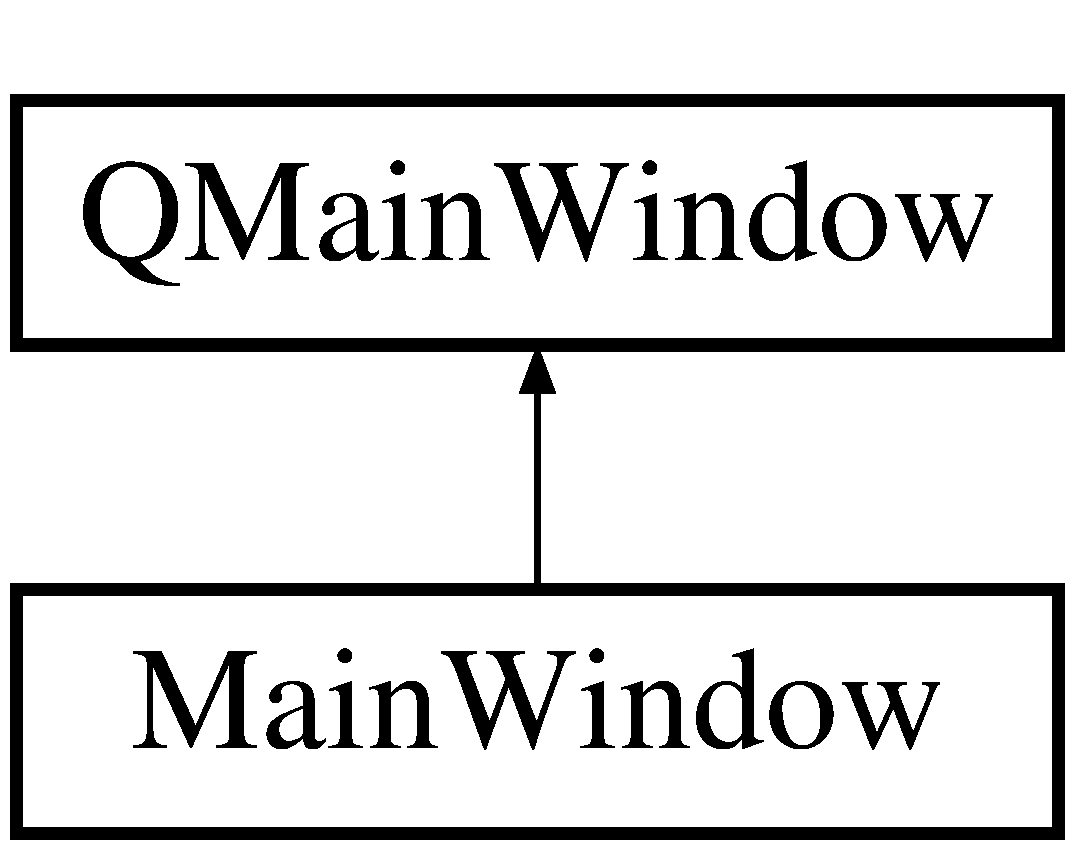
\includegraphics[height=2.000000cm]{class_main_window}
\end{center}
\end{figure}
\subsection*{Public Slots}
\begin{DoxyCompactItemize}
\item 
\mbox{\Hypertarget{class_main_window_a24cbc2d86087096b6b0212ea98008bc4}\label{class_main_window_a24cbc2d86087096b6b0212ea98008bc4}} 
void \hyperlink{class_main_window_a24cbc2d86087096b6b0212ea98008bc4}{handle\+Edit\+Dicom\+Attributes\+Button\+Clicked} ()
\begin{DoxyCompactList}\small\item\em Show the D\+I\+C\+OM attributes dialog. \end{DoxyCompactList}\item 
void \hyperlink{class_main_window_ac4c08658eff907f63479a31e94c1b76a}{handle\+Source\+Dir\+Push\+Button\+Clicked} ()
\begin{DoxyCompactList}\small\item\em handle\+Source\+Dir\+Push\+Button\+Clicked The source directory chooser button was clicked. \end{DoxyCompactList}\item 
void \hyperlink{class_main_window_a42f6da35303ef73e55320c807b598d3c}{handle\+Dest\+Dir\+Push\+Button\+Clicked} ()
\begin{DoxyCompactList}\small\item\em handle\+Destination\+Dir\+Push\+Button\+Clicked The destination directory chooser button was clicked. \end{DoxyCompactList}\item 
void \hyperlink{class_main_window_abbc2f350f4207ce69a8ce16ad4b32bb4}{handle\+Overwrite\+Files\+Check\+Box\+Clicked} (bool checked)
\begin{DoxyCompactList}\small\item\em handle\+Overwrite\+Files\+Check\+Box\+Clicked User selects whether Convert\+To\+Dicom will write into an existing directory containing files. \end{DoxyCompactList}\item 
\mbox{\Hypertarget{class_main_window_a899a5aace9eadd6146887172fb1050ed}\label{class_main_window_a899a5aace9eadd6146887172fb1050ed}} 
void \hyperlink{class_main_window_a899a5aace9eadd6146887172fb1050ed}{handle\+Convert\+Button\+Clicked} ()
\begin{DoxyCompactList}\small\item\em handle\+Convert\+Button\+Clicked Start the conversion process. \end{DoxyCompactList}\item 
void \hyperlink{class_main_window_a63e1e9e78dfd3d3e91943467ca01d2f9}{handle\+Close\+Button\+Clicked} ()
\begin{DoxyCompactList}\small\item\em handle\+Close\+Button\+Clicked \end{DoxyCompactList}\item 
\mbox{\Hypertarget{class_main_window_ab2e19e743a5f3decdc2357d38b7d0210}\label{class_main_window_ab2e19e743a5f3decdc2357d38b7d0210}} 
void \hyperlink{class_main_window_ab2e19e743a5f3decdc2357d38b7d0210}{handle\+Source\+Dir\+Line\+Edit\+Editing\+Finished} ()
\begin{DoxyCompactList}\small\item\em The user has finished editing the source directory name. \end{DoxyCompactList}\item 
\mbox{\Hypertarget{class_main_window_a2f4da079c766e6d57b985921ff0697d4}\label{class_main_window_a2f4da079c766e6d57b985921ff0697d4}} 
void \hyperlink{class_main_window_a2f4da079c766e6d57b985921ff0697d4}{handle\+Source\+Dir\+Line\+Edit\+Text\+Edited} ()
\begin{DoxyCompactList}\small\item\em The user has made an edit to the source directory name. \end{DoxyCompactList}\item 
\mbox{\Hypertarget{class_main_window_a266ea611700bed71bf603486d32d4d9e}\label{class_main_window_a266ea611700bed71bf603486d32d4d9e}} 
void \hyperlink{class_main_window_a266ea611700bed71bf603486d32d4d9e}{handle\+Dest\+Dir\+Line\+Edit\+Editing\+Finished} ()
\begin{DoxyCompactList}\small\item\em The user has finished editing the destination directory name. \end{DoxyCompactList}\item 
\mbox{\Hypertarget{class_main_window_a4aa3df85f0feb5b90bbdd62a482fc378}\label{class_main_window_a4aa3df85f0feb5b90bbdd62a482fc378}} 
void \hyperlink{class_main_window_a4aa3df85f0feb5b90bbdd62a482fc378}{handle\+Dest\+Dir\+Line\+Edit\+Text\+Edited} ()
\begin{DoxyCompactList}\small\item\em The user has made an edit to the destination directory name. \end{DoxyCompactList}\end{DoxyCompactItemize}
\subsection*{Public Member Functions}
\begin{DoxyCompactItemize}
\item 
\mbox{\Hypertarget{class_main_window_a8b244be8b7b7db1b08de2a2acb9409db}\label{class_main_window_a8b244be8b7b7db1b08de2a2acb9409db}} 
{\bfseries Main\+Window} (Q\+Widget $\ast$parent=0)
\item 
\mbox{\Hypertarget{class_main_window_a72e20beaa72b85bd6590e959f19a1a3c}\label{class_main_window_a72e20beaa72b85bd6590e959f19a1a3c}} 
void \hyperlink{class_main_window_a72e20beaa72b85bd6590e959f19a1a3c}{load\+Widget\+Info} ()
\begin{DoxyCompactList}\small\item\em load\+Widget\+Info Load values from series\+Info to the widgets on this window. \end{DoxyCompactList}\item 
\mbox{\Hypertarget{class_main_window_a8b291e7ff1acfac3e694e5773508db9e}\label{class_main_window_a8b291e7ff1acfac3e694e5773508db9e}} 
void \hyperlink{class_main_window_a8b291e7ff1acfac3e694e5773508db9e}{save\+Widget\+Info} ()
\begin{DoxyCompactList}\small\item\em save\+Widget\+Info Save values tp series\+Info from the widgets on this window. \end{DoxyCompactList}\item 
bool \hyperlink{class_main_window_a9c938dcc890c7a6d8f8df98877b1acec}{is\+Valid\+Source\+Directory} (const Q\+String \&dir\+Path)
\begin{DoxyCompactList}\small\item\em Determines whether the source directory string describes a directory containing readable image files. \end{DoxyCompactList}\item 
bool \hyperlink{class_main_window_ae3a95084dfba8d357b4dad44a97c0d75}{is\+Valid\+Dest\+Directory} (const Q\+String \&dir\+Name)
\begin{DoxyCompactList}\small\item\em Determines whether the destination directory string describes a suitable output directory. \end{DoxyCompactList}\item 
\mbox{\Hypertarget{class_main_window_a46b10fae330fb120408ff5ecf4d93917}\label{class_main_window_a46b10fae330fb120408ff5ecf4d93917}} 
void {\bfseries update\+Preview} ()
\item 
\mbox{\Hypertarget{class_main_window_a70f1571a374bc94df84f935f8af0fffe}\label{class_main_window_a70f1571a374bc94df84f935f8af0fffe}} 
void {\bfseries clear\+Preview} ()
\end{DoxyCompactItemize}


\subsection{Member Function Documentation}
\mbox{\Hypertarget{class_main_window_a63e1e9e78dfd3d3e91943467ca01d2f9}\label{class_main_window_a63e1e9e78dfd3d3e91943467ca01d2f9}} 
\index{Main\+Window@{Main\+Window}!handle\+Close\+Button\+Clicked@{handle\+Close\+Button\+Clicked}}
\index{handle\+Close\+Button\+Clicked@{handle\+Close\+Button\+Clicked}!Main\+Window@{Main\+Window}}
\subsubsection{\texorpdfstring{handle\+Close\+Button\+Clicked}{handleCloseButtonClicked}}
{\footnotesize\ttfamily void Main\+Window\+::handle\+Close\+Button\+Clicked (\begin{DoxyParamCaption}{ }\end{DoxyParamCaption})\hspace{0.3cm}{\ttfamily [slot]}}



handle\+Close\+Button\+Clicked 

\mbox{\Hypertarget{class_main_window_a42f6da35303ef73e55320c807b598d3c}\label{class_main_window_a42f6da35303ef73e55320c807b598d3c}} 
\index{Main\+Window@{Main\+Window}!handle\+Dest\+Dir\+Push\+Button\+Clicked@{handle\+Dest\+Dir\+Push\+Button\+Clicked}}
\index{handle\+Dest\+Dir\+Push\+Button\+Clicked@{handle\+Dest\+Dir\+Push\+Button\+Clicked}!Main\+Window@{Main\+Window}}
\subsubsection{\texorpdfstring{handle\+Dest\+Dir\+Push\+Button\+Clicked}{handleDestDirPushButtonClicked}}
{\footnotesize\ttfamily void Main\+Window\+::handle\+Dest\+Dir\+Push\+Button\+Clicked (\begin{DoxyParamCaption}{ }\end{DoxyParamCaption})\hspace{0.3cm}{\ttfamily [slot]}}



handle\+Destination\+Dir\+Push\+Button\+Clicked The destination directory chooser button was clicked. 

This shows a Q\+File\+Dialog. \mbox{\Hypertarget{class_main_window_abbc2f350f4207ce69a8ce16ad4b32bb4}\label{class_main_window_abbc2f350f4207ce69a8ce16ad4b32bb4}} 
\index{Main\+Window@{Main\+Window}!handle\+Overwrite\+Files\+Check\+Box\+Clicked@{handle\+Overwrite\+Files\+Check\+Box\+Clicked}}
\index{handle\+Overwrite\+Files\+Check\+Box\+Clicked@{handle\+Overwrite\+Files\+Check\+Box\+Clicked}!Main\+Window@{Main\+Window}}
\subsubsection{\texorpdfstring{handle\+Overwrite\+Files\+Check\+Box\+Clicked}{handleOverwriteFilesCheckBoxClicked}}
{\footnotesize\ttfamily void Main\+Window\+::handle\+Overwrite\+Files\+Check\+Box\+Clicked (\begin{DoxyParamCaption}\item[{bool}]{checked }\end{DoxyParamCaption})\hspace{0.3cm}{\ttfamily [slot]}}



handle\+Overwrite\+Files\+Check\+Box\+Clicked User selects whether Convert\+To\+Dicom will write into an existing directory containing files. 


\begin{DoxyParams}{Parameters}
{\em checked} & Write files into an existing directory containing files if true. Refuse otherwise. \\
\hline
\end{DoxyParams}
\mbox{\Hypertarget{class_main_window_ac4c08658eff907f63479a31e94c1b76a}\label{class_main_window_ac4c08658eff907f63479a31e94c1b76a}} 
\index{Main\+Window@{Main\+Window}!handle\+Source\+Dir\+Push\+Button\+Clicked@{handle\+Source\+Dir\+Push\+Button\+Clicked}}
\index{handle\+Source\+Dir\+Push\+Button\+Clicked@{handle\+Source\+Dir\+Push\+Button\+Clicked}!Main\+Window@{Main\+Window}}
\subsubsection{\texorpdfstring{handle\+Source\+Dir\+Push\+Button\+Clicked}{handleSourceDirPushButtonClicked}}
{\footnotesize\ttfamily void Main\+Window\+::handle\+Source\+Dir\+Push\+Button\+Clicked (\begin{DoxyParamCaption}{ }\end{DoxyParamCaption})\hspace{0.3cm}{\ttfamily [slot]}}



handle\+Source\+Dir\+Push\+Button\+Clicked The source directory chooser button was clicked. 

This shows a Q\+File\+Dialog. \mbox{\Hypertarget{class_main_window_ae3a95084dfba8d357b4dad44a97c0d75}\label{class_main_window_ae3a95084dfba8d357b4dad44a97c0d75}} 
\index{Main\+Window@{Main\+Window}!is\+Valid\+Dest\+Directory@{is\+Valid\+Dest\+Directory}}
\index{is\+Valid\+Dest\+Directory@{is\+Valid\+Dest\+Directory}!Main\+Window@{Main\+Window}}
\subsubsection{\texorpdfstring{is\+Valid\+Dest\+Directory()}{isValidDestDirectory()}}
{\footnotesize\ttfamily bool Main\+Window\+::is\+Valid\+Dest\+Directory (\begin{DoxyParamCaption}\item[{const Q\+String \&}]{dir\+Name }\end{DoxyParamCaption})}



Determines whether the destination directory string describes a suitable output directory. 

The directory must exist (or be creatable) and be writeable. If the directory is not empty and series\+Info-\/$>$overwrite\+Files() is false we will refuse to write to the directory. Otherwise the files will be written, overwriting any that are in he way. 
\begin{DoxyParams}{Parameters}
{\em dir\+Name} & The directory to be tested. \\
\hline
\end{DoxyParams}
\begin{DoxyReturn}{Returns}
true if valid, false if not. 
\end{DoxyReturn}
\mbox{\Hypertarget{class_main_window_a9c938dcc890c7a6d8f8df98877b1acec}\label{class_main_window_a9c938dcc890c7a6d8f8df98877b1acec}} 
\index{Main\+Window@{Main\+Window}!is\+Valid\+Source\+Directory@{is\+Valid\+Source\+Directory}}
\index{is\+Valid\+Source\+Directory@{is\+Valid\+Source\+Directory}!Main\+Window@{Main\+Window}}
\subsubsection{\texorpdfstring{is\+Valid\+Source\+Directory()}{isValidSourceDirectory()}}
{\footnotesize\ttfamily bool Main\+Window\+::is\+Valid\+Source\+Directory (\begin{DoxyParamCaption}\item[{const Q\+String \&}]{dir\+Path }\end{DoxyParamCaption})}



Determines whether the source directory string describes a directory containing readable image files. 


\begin{DoxyParams}{Parameters}
{\em dir\+Path} & The directory to be tested. \\
\hline
\end{DoxyParams}
\begin{DoxyReturn}{Returns}
true if valid, false if not. 
\end{DoxyReturn}


The documentation for this class was generated from the following files\+:\begin{DoxyCompactItemize}
\item 
mainwindow.\+h\item 
mainwindow.\+cpp\end{DoxyCompactItemize}

\hypertarget{class_series_converter}{}\section{Series\+Converter Class Reference}
\label{class_series_converter}\index{Series\+Converter@{Series\+Converter}}


The \hyperlink{class_series_converter}{Series\+Converter} class.  




{\ttfamily \#include $<$seriesconverter.\+h$>$}

\subsection*{Public Member Functions}
\begin{DoxyCompactItemize}
\item 
\mbox{\Hypertarget{class_series_converter_a807a4cbcfab6044a4635f72b72d6a0d3}\label{class_series_converter_a807a4cbcfab6044a4635f72b72d6a0d3}} 
\hyperlink{class_series_converter_a807a4cbcfab6044a4635f72b72d6a0d3}{Series\+Converter} ()
\begin{DoxyCompactList}\small\item\em \hyperlink{class_series_converter}{Series\+Converter} Constructor. \end{DoxyCompactList}\item 
Error\+Code \hyperlink{class_series_converter_ac8729b482ee4eda39bd6a9e710f4449c}{convert\+Files} ()
\begin{DoxyCompactList}\small\item\em Read the input files and write the D\+I\+C\+OM files to the output directory. \end{DoxyCompactList}\item 
Error\+Code \hyperlink{class_series_converter_a1c8cd4b434f931afdbd719375aa64904}{make\+Full\+Output\+Path\+Dir} (const Q\+String \&dir\+Name)
\begin{DoxyCompactList}\small\item\em Make the full output directory path. \end{DoxyCompactList}\item 
void \hyperlink{class_series_converter_aeae7772dca9eaa2ad685cb7c3b79dbf0}{set\+Input\+Dir} (const Q\+Dir \&dir)
\begin{DoxyCompactList}\small\item\em set\+Input\+Dir \end{DoxyCompactList}\item 
Error\+Code \hyperlink{class_series_converter_af4bcee40f249309b5b153fc951196ddb}{extract\+Image\+Parameters} ()
\begin{DoxyCompactList}\small\item\em Tries to get as many metadata from the input image files as possible. \end{DoxyCompactList}\item 
bool \hyperlink{class_series_converter_a88356a78d84c2d3aba7f4a340c4202ed}{is\+Valid\+Source\+Dir} (const Q\+String \&dir\+Path)
\begin{DoxyCompactList}\small\item\em Determines whether a directory is a valid souurce directory. \end{DoxyCompactList}\end{DoxyCompactItemize}


\subsection{Detailed Description}
The \hyperlink{class_series_converter}{Series\+Converter} class. 

Class to do the conversion of one series. It reads the image files, converts them to D\+I\+C\+OM and writes them out as D\+I\+C\+OM files. 

\subsection{Member Function Documentation}
\mbox{\Hypertarget{class_series_converter_ac8729b482ee4eda39bd6a9e710f4449c}\label{class_series_converter_ac8729b482ee4eda39bd6a9e710f4449c}} 
\index{Series\+Converter@{Series\+Converter}!convert\+Files@{convert\+Files}}
\index{convert\+Files@{convert\+Files}!Series\+Converter@{Series\+Converter}}
\subsubsection{\texorpdfstring{convert\+Files()}{convertFiles()}}
{\footnotesize\ttfamily Error\+Code Series\+Converter\+::convert\+Files (\begin{DoxyParamCaption}{ }\end{DoxyParamCaption})}



Read the input files and write the D\+I\+C\+OM files to the output directory. 

A directory tree is formed like this\+: patients\+Name/study\+Description -\/ study\+I\+D/series\+Description -\/ series\+Number. \begin{DoxyReturn}{Returns}
Suitable code in Error\+Code enum. 
\end{DoxyReturn}
\mbox{\Hypertarget{class_series_converter_af4bcee40f249309b5b153fc951196ddb}\label{class_series_converter_af4bcee40f249309b5b153fc951196ddb}} 
\index{Series\+Converter@{Series\+Converter}!extract\+Image\+Parameters@{extract\+Image\+Parameters}}
\index{extract\+Image\+Parameters@{extract\+Image\+Parameters}!Series\+Converter@{Series\+Converter}}
\subsubsection{\texorpdfstring{extract\+Image\+Parameters()}{extractImageParameters()}}
{\footnotesize\ttfamily Error\+Code Series\+Converter\+::extract\+Image\+Parameters (\begin{DoxyParamCaption}{ }\end{DoxyParamCaption})}



Tries to get as many metadata from the input image files as possible. 

If the image is a D\+I\+C\+OM series the metadata dictionary will be queried. Otherwise the data will likely be limited to dimensions and slice spacing. This must be called after read\+Files(). \begin{DoxyReturn}{Returns}
Suitable code in Error\+Code enum. 
\end{DoxyReturn}
\mbox{\Hypertarget{class_series_converter_a88356a78d84c2d3aba7f4a340c4202ed}\label{class_series_converter_a88356a78d84c2d3aba7f4a340c4202ed}} 
\index{Series\+Converter@{Series\+Converter}!is\+Valid\+Source\+Dir@{is\+Valid\+Source\+Dir}}
\index{is\+Valid\+Source\+Dir@{is\+Valid\+Source\+Dir}!Series\+Converter@{Series\+Converter}}
\subsubsection{\texorpdfstring{is\+Valid\+Source\+Dir()}{isValidSourceDir()}}
{\footnotesize\ttfamily bool Series\+Converter\+::is\+Valid\+Source\+Dir (\begin{DoxyParamCaption}\item[{const Q\+String \&}]{dir\+Path }\end{DoxyParamCaption})}



Determines whether a directory is a valid souurce directory. 


\begin{DoxyParams}{Parameters}
{\em dir\+Path} & The path of the directory. \\
\hline
\end{DoxyParams}
\begin{DoxyReturn}{Returns}
true if we can use dir\+Path, false otherwise. 
\end{DoxyReturn}
\mbox{\Hypertarget{class_series_converter_a1c8cd4b434f931afdbd719375aa64904}\label{class_series_converter_a1c8cd4b434f931afdbd719375aa64904}} 
\index{Series\+Converter@{Series\+Converter}!make\+Full\+Output\+Path\+Dir@{make\+Full\+Output\+Path\+Dir}}
\index{make\+Full\+Output\+Path\+Dir@{make\+Full\+Output\+Path\+Dir}!Series\+Converter@{Series\+Converter}}
\subsubsection{\texorpdfstring{make\+Full\+Output\+Path\+Dir()}{makeFullOutputPathDir()}}
{\footnotesize\ttfamily Error\+Code Series\+Converter\+::make\+Full\+Output\+Path\+Dir (\begin{DoxyParamCaption}\item[{const Q\+String \&}]{dir\+Name }\end{DoxyParamCaption})}



Make the full output directory path. 

This is the directory into which the D\+I\+C\+OM series will be placed. 
\begin{DoxyParams}{Parameters}
{\em dir\+Name} & The output directory name that will be expanded by make\+Output\+Path\+Name(). \\
\hline
\end{DoxyParams}
\begin{DoxyReturn}{Returns}
Error\+Code S\+U\+C\+C\+E\+SS if successful, E\+R\+R\+O\+R\+\_\+\+C\+R\+E\+A\+T\+I\+N\+G\+\_\+\+D\+I\+R\+E\+C\+T\+O\+RY or E\+R\+R\+O\+R\+\_\+\+D\+I\+R\+E\+C\+T\+O\+R\+Y\+\_\+\+N\+O\+T\+\_\+\+E\+M\+P\+TY if not. 
\end{DoxyReturn}
\mbox{\Hypertarget{class_series_converter_aeae7772dca9eaa2ad685cb7c3b79dbf0}\label{class_series_converter_aeae7772dca9eaa2ad685cb7c3b79dbf0}} 
\index{Series\+Converter@{Series\+Converter}!set\+Input\+Dir@{set\+Input\+Dir}}
\index{set\+Input\+Dir@{set\+Input\+Dir}!Series\+Converter@{Series\+Converter}}
\subsubsection{\texorpdfstring{set\+Input\+Dir()}{setInputDir()}}
{\footnotesize\ttfamily void Series\+Converter\+::set\+Input\+Dir (\begin{DoxyParamCaption}\item[{const Q\+Dir \&}]{dir }\end{DoxyParamCaption})\hspace{0.3cm}{\ttfamily [inline]}}



set\+Input\+Dir 


\begin{DoxyParams}{Parameters}
{\em dir} & The directory containing the files to be read. Tells us where the files are. \\
\hline
\end{DoxyParams}


The documentation for this class was generated from the following files\+:\begin{DoxyCompactItemize}
\item 
seriesconverter.\+h\item 
seriesconverter.\+cpp\end{DoxyCompactItemize}

\hypertarget{class_series_info}{}\section{Series\+Info Class Reference}
\label{class_series_info}\index{Series\+Info@{Series\+Info}}


The \hyperlink{class_series_info}{Series\+Info} class This class contains all of the D\+I\+C\+OM and other information needed to do the conversions.  




{\ttfamily \#include $<$seriesinfo.\+h$>$}

\subsection*{Public Member Functions}
\begin{DoxyCompactItemize}
\item 
bool \hyperlink{class_series_info_a21fe1bd18d2f9e2b1f7ceb22e7ad98a3}{overwrite\+Files} () const
\begin{DoxyCompactList}\small\item\em overwrite\+Files Get flag which indicates whether generated files will overwrite existing files. \end{DoxyCompactList}\item 
Q\+Dir \hyperlink{class_series_info_ab30b8c01a3413b913f00203b2ef5a117}{input\+Dir} () const
\begin{DoxyCompactList}\small\item\em input\+Dir Get the directory containing the files to be converted. \end{DoxyCompactList}\item 
Q\+String \hyperlink{class_series_info_a550fbfcf3061fdd50850baa788bf376d}{input\+Dir\+Str} () const
\begin{DoxyCompactList}\small\item\em input\+Dir\+Str \end{DoxyCompactList}\item 
Q\+Dir \hyperlink{class_series_info_af94b9048bc3b60b5d151f227299b394b}{output\+Dir} () const
\begin{DoxyCompactList}\small\item\em output\+Dir This is a base subdirectory for the output of this program. \end{DoxyCompactList}\item 
Q\+String \hyperlink{class_series_info_abc897c5c859293338e45d193ac62c674}{output\+Dir\+Str} () const
\begin{DoxyCompactList}\small\item\em output\+Dir\+Str \end{DoxyCompactList}\item 
Q\+String \hyperlink{class_series_info_a7088530574522d3d1123806c766402f2}{output\+Path} () const
\begin{DoxyCompactList}\small\item\em output\+Path The full output path is a chain of subdirectories of based upon \hyperlink{class_series_info_abc897c5c859293338e45d193ac62c674}{output\+Dir\+Str()}, patient\textquotesingle{}s name, study description, study ID, series description and series number. \end{DoxyCompactList}\item 
\mbox{\Hypertarget{class_series_info_ae6eda4a724007bddd85b5b6832648590}\label{class_series_info_ae6eda4a724007bddd85b5b6832648590}} 
Q\+String {\bfseries patient\+Name} () const
\item 
\mbox{\Hypertarget{class_series_info_a5b04d7095b2bf6728bc02e5f5fd9964a}\label{class_series_info_a5b04d7095b2bf6728bc02e5f5fd9964a}} 
Q\+String {\bfseries patient\+ID} () const
\item 
\mbox{\Hypertarget{class_series_info_a6718f39279d903a522c6c7e6dc9558b7}\label{class_series_info_a6718f39279d903a522c6c7e6dc9558b7}} 
Q\+Date {\bfseries patient\+D\+OB} () const
\item 
\mbox{\Hypertarget{class_series_info_ad2d4cfc6d71e16b8f44910937dad7d8a}\label{class_series_info_ad2d4cfc6d71e16b8f44910937dad7d8a}} 
Q\+String {\bfseries patient\+D\+O\+B\+Str} () const
\item 
\mbox{\Hypertarget{class_series_info_a4330c792ea2a959d442139856afe783d}\label{class_series_info_a4330c792ea2a959d442139856afe783d}} 
Q\+String {\bfseries patient\+Sex} () const
\item 
\mbox{\Hypertarget{class_series_info_af6564a18ffa1fbddcf32d273dac430f9}\label{class_series_info_af6564a18ffa1fbddcf32d273dac430f9}} 
Q\+String {\bfseries study\+Description} () const
\item 
\mbox{\Hypertarget{class_series_info_ac29186ca4e8d7703dbf2da4dac3871cf}\label{class_series_info_ac29186ca4e8d7703dbf2da4dac3871cf}} 
Q\+String {\bfseries study\+ID} () const
\item 
\mbox{\Hypertarget{class_series_info_ad6b4be6ab8b9c1bf2377e98c5d1ffb31}\label{class_series_info_ad6b4be6ab8b9c1bf2377e98c5d1ffb31}} 
Q\+String {\bfseries study\+Modality} () const
\item 
\mbox{\Hypertarget{class_series_info_a2eb0ac1652fc77f6d9d9bcfcae33c5af}\label{class_series_info_a2eb0ac1652fc77f6d9d9bcfcae33c5af}} 
Q\+Date\+Time {\bfseries study\+Date\+Time} () const
\item 
\mbox{\Hypertarget{class_series_info_a99cc72da568ff148637b5f4dff5252c0}\label{class_series_info_a99cc72da568ff148637b5f4dff5252c0}} 
Q\+String {\bfseries study\+Date\+Time\+Str} () const
\item 
\mbox{\Hypertarget{class_series_info_a2decc9e9c01f7a9fc27c6a88f0871039}\label{class_series_info_a2decc9e9c01f7a9fc27c6a88f0871039}} 
Q\+String {\bfseries study\+Instance\+U\+ID} () const
\item 
\mbox{\Hypertarget{class_series_info_a77d678e8efd4564738cdbd1e7accec11}\label{class_series_info_a77d678e8efd4564738cdbd1e7accec11}} 
int {\bfseries series\+Number} () const
\item 
\mbox{\Hypertarget{class_series_info_a5d1cbb206f2ea1c9873ab0b8137ccda1}\label{class_series_info_a5d1cbb206f2ea1c9873ab0b8137ccda1}} 
Q\+String {\bfseries series\+Number\+Str} () const
\item 
\mbox{\Hypertarget{class_series_info_a713638b77beb8e167bbd55a23e289ec6}\label{class_series_info_a713638b77beb8e167bbd55a23e289ec6}} 
Q\+String {\bfseries series\+Description} () const
\item 
\mbox{\Hypertarget{class_series_info_a631bbb07847fdaab973df74f6f052b0e}\label{class_series_info_a631bbb07847fdaab973df74f6f052b0e}} 
Q\+String {\bfseries series\+Position\+Patient} () const
\item 
double \hyperlink{class_series_info_aa3cd8fea1ca4d619817e07be017fb7d6}{series\+Time\+Increment} () const
\begin{DoxyCompactList}\small\item\em series\+Time\+Increment \end{DoxyCompactList}\item 
\mbox{\Hypertarget{class_series_info_af1da8f078d398e0ab3fc8f5129518e0b}\label{class_series_info_af1da8f078d398e0ab3fc8f5129518e0b}} 
Q\+String {\bfseries series\+Time\+Increment\+Str} () const
\item 
\mbox{\Hypertarget{class_series_info_a94facc78d30d5daeb6ae28fbdd824c77}\label{class_series_info_a94facc78d30d5daeb6ae28fbdd824c77}} 
Q\+List$<$ Q\+Time $>$ \& {\bfseries acq\+Times} ()
\item 
\mbox{\Hypertarget{class_series_info_ab6e94bbff402e228a7b680d32d2d1a66}\label{class_series_info_ab6e94bbff402e228a7b680d32d2d1a66}} 
int {\bfseries image\+Number\+Of\+Images} () const
\item 
\mbox{\Hypertarget{class_series_info_a2f21da996a318aec02438d5f7d7dd350}\label{class_series_info_a2f21da996a318aec02438d5f7d7dd350}} 
Q\+String {\bfseries image\+Number\+Of\+Images\+Str} () const
\item 
\mbox{\Hypertarget{class_series_info_a595cb840a0fe00e330d58bee0161ba62}\label{class_series_info_a595cb840a0fe00e330d58bee0161ba62}} 
int {\bfseries image\+Slices\+Per\+Image} () const
\item 
\mbox{\Hypertarget{class_series_info_a67207f1efd50367b46d946129fb6dfe1}\label{class_series_info_a67207f1efd50367b46d946129fb6dfe1}} 
Q\+String {\bfseries image\+Slices\+Per\+Image\+Str} () const
\item 
\mbox{\Hypertarget{class_series_info_ae7a7057c7d20f59650077dfa52dec97d}\label{class_series_info_ae7a7057c7d20f59650077dfa52dec97d}} 
int {\bfseries image\+Number\+Of\+Slices} () const
\item 
\mbox{\Hypertarget{class_series_info_ac8697c73a137e9047033e33b6352568b}\label{class_series_info_ac8697c73a137e9047033e33b6352568b}} 
Q\+String {\bfseries image\+Number\+Of\+Slices\+Str} () const
\item 
\mbox{\Hypertarget{class_series_info_a7ac539de8bcb047280dd0ae04c1ff876}\label{class_series_info_a7ac539de8bcb047280dd0ae04c1ff876}} 
double {\bfseries image\+Slice\+Spacing} () const
\item 
\mbox{\Hypertarget{class_series_info_adc5abb8c7656afc0ecf15eb4436ae712}\label{class_series_info_adc5abb8c7656afc0ecf15eb4436ae712}} 
Q\+String {\bfseries image\+Slice\+Spacing\+Str} () const
\item 
\mbox{\Hypertarget{class_series_info_a91685a94ead368bbb9b1cd697d0e5c59}\label{class_series_info_a91685a94ead368bbb9b1cd697d0e5c59}} 
double {\bfseries image\+Position\+PatientX} () const
\item 
\mbox{\Hypertarget{class_series_info_a3d273fccf13a4a3c84ba53bc545f4641}\label{class_series_info_a3d273fccf13a4a3c84ba53bc545f4641}} 
Q\+String {\bfseries image\+Position\+Patient\+X\+Str} () const
\item 
\mbox{\Hypertarget{class_series_info_a63f3d9368ab755c8a7f6d7e54d03c09d}\label{class_series_info_a63f3d9368ab755c8a7f6d7e54d03c09d}} 
double {\bfseries image\+Position\+PatientY} () const
\item 
\mbox{\Hypertarget{class_series_info_ae7e8c788abaf34369ce8cd360653a2f5}\label{class_series_info_ae7e8c788abaf34369ce8cd360653a2f5}} 
Q\+String {\bfseries image\+Position\+Patient\+Y\+Str} () const
\item 
\mbox{\Hypertarget{class_series_info_a5a53ec11248767dc34393520ddc64d81}\label{class_series_info_a5a53ec11248767dc34393520ddc64d81}} 
double {\bfseries image\+Position\+PatientZ} () const
\item 
\mbox{\Hypertarget{class_series_info_afd3b1a76c1f8986a5a787e2909df8b3f}\label{class_series_info_afd3b1a76c1f8986a5a787e2909df8b3f}} 
Q\+String {\bfseries image\+Position\+Patient\+Z\+Str} () const
\item 
\mbox{\Hypertarget{class_series_info_ab31237968717e9c71d21d20a3929d115}\label{class_series_info_ab31237968717e9c71d21d20a3929d115}} 
Q\+String {\bfseries image\+Patient\+Orientation} () const
\item 
void \hyperlink{class_series_info_a09ff36a5e9ad4ec4cd2030a8e5abefa2}{set\+Overwrite\+Files} (bool \hyperlink{class_series_info_a21fe1bd18d2f9e2b1f7ceb22e7ad98a3}{overwrite\+Files})
\begin{DoxyCompactList}\small\item\em set\+Overwrite\+Files Set flag which indicates whether generated files will overwrite existing files. \end{DoxyCompactList}\item 
void \hyperlink{class_series_info_a19ce250d3f423a513a6492b9bd5aa908}{set\+Input\+Dir} (const Q\+Dir \&\hyperlink{class_series_info_ab30b8c01a3413b913f00203b2ef5a117}{input\+Dir})
\begin{DoxyCompactList}\small\item\em set\+Input\+Dir Set the input directory path \end{DoxyCompactList}\item 
\mbox{\Hypertarget{class_series_info_acf0f521d849807a9382fa791bf745482}\label{class_series_info_acf0f521d849807a9382fa791bf745482}} 
void {\bfseries set\+Output\+Dir} (const Q\+Dir \&\hyperlink{class_series_info_af94b9048bc3b60b5d151f227299b394b}{output\+Dir})
\item 
\mbox{\Hypertarget{class_series_info_a2124d48ae7a2b09d99f7a3e3e67155f2}\label{class_series_info_a2124d48ae7a2b09d99f7a3e3e67155f2}} 
void {\bfseries set\+Output\+Path} (const Q\+String \&\hyperlink{class_series_info_a7088530574522d3d1123806c766402f2}{output\+Path})
\item 
\mbox{\Hypertarget{class_series_info_ad94c20360198b39fd185cf77a158e4b3}\label{class_series_info_ad94c20360198b39fd185cf77a158e4b3}} 
void {\bfseries set\+Image\+Number\+Of\+Images} (int number\+Of\+Images)
\item 
\mbox{\Hypertarget{class_series_info_ac3bc2f9b3b730ca1f6d9f5ee4f26d6ba}\label{class_series_info_ac3bc2f9b3b730ca1f6d9f5ee4f26d6ba}} 
void {\bfseries set\+Image\+Slices\+Per\+Image} (int slices\+Per\+Image)
\item 
\mbox{\Hypertarget{class_series_info_ac6040514bc12b33a27508e393a47ad15}\label{class_series_info_ac6040514bc12b33a27508e393a47ad15}} 
void {\bfseries set\+Series\+Number\+Of\+Slices} (int number\+Of\+Slices)
\item 
\mbox{\Hypertarget{class_series_info_ab47d111e20b8f0cc53a55518930efd6f}\label{class_series_info_ab47d111e20b8f0cc53a55518930efd6f}} 
void {\bfseries set\+Patient\+Name} (const Q\+String \&patient\+Name)
\item 
\mbox{\Hypertarget{class_series_info_a489836b82b5ed54f307fd850369c3939}\label{class_series_info_a489836b82b5ed54f307fd850369c3939}} 
void {\bfseries set\+Patient\+ID} (const Q\+String \&patient\+ID)
\item 
\mbox{\Hypertarget{class_series_info_aeae3148f709f152b9705f7e4524e8506}\label{class_series_info_aeae3148f709f152b9705f7e4524e8506}} 
void {\bfseries set\+Patient\+D\+OB} (const Q\+Date \&patient\+D\+OB)
\item 
\mbox{\Hypertarget{class_series_info_a5f3e8081e83919e79577942b6b03033b}\label{class_series_info_a5f3e8081e83919e79577942b6b03033b}} 
void {\bfseries set\+Patient\+Sex} (const Q\+String \&patient\+Sex)
\item 
\mbox{\Hypertarget{class_series_info_ada0323bceb521e6bce25fe2d9db76493}\label{class_series_info_ada0323bceb521e6bce25fe2d9db76493}} 
void {\bfseries set\+Study\+Description} (const Q\+String \&study\+Description)
\item 
\mbox{\Hypertarget{class_series_info_ab9581aedaafd907979bf3f4f8f3a4eec}\label{class_series_info_ab9581aedaafd907979bf3f4f8f3a4eec}} 
void {\bfseries set\+Study\+ID} (const Q\+String \&study\+ID)
\item 
\mbox{\Hypertarget{class_series_info_a4c6efd5f4a4c884389ce27e88c375591}\label{class_series_info_a4c6efd5f4a4c884389ce27e88c375591}} 
void {\bfseries set\+Study\+Modality} (const Q\+String \&study\+Modality)
\item 
\mbox{\Hypertarget{class_series_info_a89b29213e8130a7804f51dcb5763aeec}\label{class_series_info_a89b29213e8130a7804f51dcb5763aeec}} 
void {\bfseries set\+Study\+Date\+Time} (const Q\+Date\+Time \&study\+Date\+Time)
\item 
\mbox{\Hypertarget{class_series_info_a161916424ebbbc0525f07b06be33ab15}\label{class_series_info_a161916424ebbbc0525f07b06be33ab15}} 
void {\bfseries set\+Study\+Instance\+U\+ID} (const Q\+String \&study\+Instance\+U\+ID)
\item 
\mbox{\Hypertarget{class_series_info_a1745cd80a9707532c530f9128b1c2bc0}\label{class_series_info_a1745cd80a9707532c530f9128b1c2bc0}} 
void {\bfseries set\+Series\+Number} (const Q\+String \&series\+Number)
\item 
\mbox{\Hypertarget{class_series_info_a5fcc71c04f2a3389bf323d8a1f2e2c48}\label{class_series_info_a5fcc71c04f2a3389bf323d8a1f2e2c48}} 
void {\bfseries set\+Series\+Number} (int series\+Number)
\item 
\mbox{\Hypertarget{class_series_info_a80045682d0da7012141780b03325cea5}\label{class_series_info_a80045682d0da7012141780b03325cea5}} 
void {\bfseries set\+Series\+Description} (const Q\+String \&series\+Description)
\item 
\mbox{\Hypertarget{class_series_info_ac1600dfc5f367a0c940c28c07dfba526}\label{class_series_info_ac1600dfc5f367a0c940c28c07dfba526}} 
void {\bfseries set\+Series\+Position\+Patient} (const Q\+String \&series\+Position\+Patient)
\item 
void \hyperlink{class_series_info_aacffddaa0cdb2dd931b89e57d429912e}{set\+Series\+Time\+Increment} (double time\+Increment)
\begin{DoxyCompactList}\small\item\em set\+Series\+Time\+Increment \end{DoxyCompactList}\item 
\mbox{\Hypertarget{class_series_info_aedd83f1d0f57fe35ea8f8148205d974e}\label{class_series_info_aedd83f1d0f57fe35ea8f8148205d974e}} 
void {\bfseries set\+Image\+Slice\+Spacing} (double image\+Slice\+Spacing)
\item 
\mbox{\Hypertarget{class_series_info_a7d8d7d402a289198ff7412cbe02ec8c5}\label{class_series_info_a7d8d7d402a289198ff7412cbe02ec8c5}} 
void {\bfseries set\+Image\+Position\+PatientX} (double image\+Position\+PatientX)
\item 
\mbox{\Hypertarget{class_series_info_ae68eebb709fc373f180928bbce3fd0a5}\label{class_series_info_ae68eebb709fc373f180928bbce3fd0a5}} 
void {\bfseries set\+Image\+Position\+PatientY} (double image\+Position\+PatientY)
\item 
\mbox{\Hypertarget{class_series_info_aa4ce9146cead6bfc3e01d99e1ecbca40}\label{class_series_info_aa4ce9146cead6bfc3e01d99e1ecbca40}} 
void {\bfseries set\+Image\+Position\+PatientZ} (double image\+Position\+PatientZ)
\item 
\mbox{\Hypertarget{class_series_info_afd896e51680aa3bc2ca55128c525ca38}\label{class_series_info_afd896e51680aa3bc2ca55128c525ca38}} 
void {\bfseries set\+Image\+Patient\+Orientation} (const Q\+String \&image\+Orientation\+Patient)
\item 
\mbox{\Hypertarget{class_series_info_a32d3ea80ee92f8b5343032083c49329b}\label{class_series_info_a32d3ea80ee92f8b5343032083c49329b}} 
void \hyperlink{class_series_info_a32d3ea80ee92f8b5343032083c49329b}{load\+Settings} ()
\begin{DoxyCompactList}\small\item\em load\+Settings Fills a data structure using the saved settings. \end{DoxyCompactList}\item 
\mbox{\Hypertarget{class_series_info_a2227e5c01d043f356219e83cbe0384c0}\label{class_series_info_a2227e5c01d043f356219e83cbe0384c0}} 
void \hyperlink{class_series_info_a2227e5c01d043f356219e83cbe0384c0}{save\+Settings} ()
\begin{DoxyCompactList}\small\item\em save\+Settings Saves the contents of info to persistent storage. \end{DoxyCompactList}\item 
bool \hyperlink{class_series_info_a3765099ab2658fa04ea0863f0b1e4b2b}{is\+Conistent} ()
\begin{DoxyCompactList}\small\item\em Check for internal completeness and conistency. \end{DoxyCompactList}\item 
itk\+::\+Meta\+Data\+Dictionary \hyperlink{class_series_info_a3855143383f2a9c6c66a05946e51d1f6}{meta\+Data\+Dictionary} () const
\begin{DoxyCompactList}\small\item\em Get the parameters as a D\+I\+C\+OM dictionary. \end{DoxyCompactList}\item 
Q\+String \hyperlink{class_series_info_ae0d61a82f9fe9caed2832478c2a2ed35}{image\+Position\+Patient\+String} () const
\begin{DoxyCompactList}\small\item\em image\+Position\+Patient\+String \end{DoxyCompactList}\item 
Q\+String \hyperlink{class_series_info_ae1484c1360ac3b7590eb938d8d5489ce}{image\+Position\+Patient\+String} (int slice\+Idx) const
\begin{DoxyCompactList}\small\item\em image\+Position\+Patient\+String \end{DoxyCompactList}\end{DoxyCompactItemize}
\subsection*{Static Public Member Functions}
\begin{DoxyCompactItemize}
\item 
static \hyperlink{class_series_info}{Series\+Info} $\ast$ \hyperlink{class_series_info_a1563e01e8605ce20c0f81976d7e729b4}{get\+Instance} ()
\begin{DoxyCompactList}\small\item\em Get the global instance of this class. \end{DoxyCompactList}\item 
static \hyperlink{class_series_info}{Series\+Info} $\ast$ \hyperlink{class_series_info_a8895ba10eb144998e6d15d57524f8ec1}{get\+Temp\+Instance} ()
\begin{DoxyCompactList}\small\item\em Get a tempory instance of this class. \end{DoxyCompactList}\end{DoxyCompactItemize}


\subsection{Detailed Description}
The \hyperlink{class_series_info}{Series\+Info} class This class contains all of the D\+I\+C\+OM and other information needed to do the conversions. 

It is set up as a singleton class because only one should ever be created and it allows the instance to be accessed globally. 

\subsection{Member Function Documentation}
\mbox{\Hypertarget{class_series_info_a1563e01e8605ce20c0f81976d7e729b4}\label{class_series_info_a1563e01e8605ce20c0f81976d7e729b4}} 
\index{Series\+Info@{Series\+Info}!get\+Instance@{get\+Instance}}
\index{get\+Instance@{get\+Instance}!Series\+Info@{Series\+Info}}
\subsubsection{\texorpdfstring{get\+Instance()}{getInstance()}}
{\footnotesize\ttfamily static \hyperlink{class_series_info}{Series\+Info}$\ast$ Series\+Info\+::get\+Instance (\begin{DoxyParamCaption}{ }\end{DoxyParamCaption})\hspace{0.3cm}{\ttfamily [inline]}, {\ttfamily [static]}}



Get the global instance of this class. 

\begin{DoxyReturn}{Returns}
Pointer to single instance of this class. 
\end{DoxyReturn}
\mbox{\Hypertarget{class_series_info_a8895ba10eb144998e6d15d57524f8ec1}\label{class_series_info_a8895ba10eb144998e6d15d57524f8ec1}} 
\index{Series\+Info@{Series\+Info}!get\+Temp\+Instance@{get\+Temp\+Instance}}
\index{get\+Temp\+Instance@{get\+Temp\+Instance}!Series\+Info@{Series\+Info}}
\subsubsection{\texorpdfstring{get\+Temp\+Instance()}{getTempInstance()}}
{\footnotesize\ttfamily static \hyperlink{class_series_info}{Series\+Info}$\ast$ Series\+Info\+::get\+Temp\+Instance (\begin{DoxyParamCaption}{ }\end{DoxyParamCaption})\hspace{0.3cm}{\ttfamily [inline]}, {\ttfamily [static]}}



Get a tempory instance of this class. 

The new instance is a copy of the global instance. \begin{DoxyReturn}{Returns}
Pointer to a temporary instance of this class. It must be {\ttfamily delete}d when no longer needed. 
\end{DoxyReturn}
\mbox{\Hypertarget{class_series_info_ae0d61a82f9fe9caed2832478c2a2ed35}\label{class_series_info_ae0d61a82f9fe9caed2832478c2a2ed35}} 
\index{Series\+Info@{Series\+Info}!image\+Position\+Patient\+String@{image\+Position\+Patient\+String}}
\index{image\+Position\+Patient\+String@{image\+Position\+Patient\+String}!Series\+Info@{Series\+Info}}
\subsubsection{\texorpdfstring{image\+Position\+Patient\+String()}{imagePositionPatientString()}\hspace{0.1cm}{\footnotesize\ttfamily [1/2]}}
{\footnotesize\ttfamily Q\+String Series\+Info\+::image\+Position\+Patient\+String (\begin{DoxyParamCaption}{ }\end{DoxyParamCaption}) const}



image\+Position\+Patient\+String 

\begin{DoxyReturn}{Returns}
The Image\+Position\+Patient as a D\+I\+C\+OM compatible string. 
\end{DoxyReturn}
\mbox{\Hypertarget{class_series_info_ae1484c1360ac3b7590eb938d8d5489ce}\label{class_series_info_ae1484c1360ac3b7590eb938d8d5489ce}} 
\index{Series\+Info@{Series\+Info}!image\+Position\+Patient\+String@{image\+Position\+Patient\+String}}
\index{image\+Position\+Patient\+String@{image\+Position\+Patient\+String}!Series\+Info@{Series\+Info}}
\subsubsection{\texorpdfstring{image\+Position\+Patient\+String()}{imagePositionPatientString()}\hspace{0.1cm}{\footnotesize\ttfamily [2/2]}}
{\footnotesize\ttfamily Q\+String Series\+Info\+::image\+Position\+Patient\+String (\begin{DoxyParamCaption}\item[{int}]{slice\+Idx }\end{DoxyParamCaption}) const}



image\+Position\+Patient\+String 


\begin{DoxyParams}{Parameters}
{\em slice\+Idx} & The slice whose position we want. \\
\hline
\end{DoxyParams}
\begin{DoxyReturn}{Returns}
The Image\+Position\+Patient for this slice as a D\+I\+C\+OM compatible string. 
\end{DoxyReturn}
\mbox{\Hypertarget{class_series_info_ab30b8c01a3413b913f00203b2ef5a117}\label{class_series_info_ab30b8c01a3413b913f00203b2ef5a117}} 
\index{Series\+Info@{Series\+Info}!input\+Dir@{input\+Dir}}
\index{input\+Dir@{input\+Dir}!Series\+Info@{Series\+Info}}
\subsubsection{\texorpdfstring{input\+Dir()}{inputDir()}}
{\footnotesize\ttfamily Q\+Dir Series\+Info\+::input\+Dir (\begin{DoxyParamCaption}{ }\end{DoxyParamCaption}) const\hspace{0.3cm}{\ttfamily [inline]}}



input\+Dir Get the directory containing the files to be converted. 

\begin{DoxyReturn}{Returns}
The current input directory. 
\end{DoxyReturn}
\mbox{\Hypertarget{class_series_info_a550fbfcf3061fdd50850baa788bf376d}\label{class_series_info_a550fbfcf3061fdd50850baa788bf376d}} 
\index{Series\+Info@{Series\+Info}!input\+Dir\+Str@{input\+Dir\+Str}}
\index{input\+Dir\+Str@{input\+Dir\+Str}!Series\+Info@{Series\+Info}}
\subsubsection{\texorpdfstring{input\+Dir\+Str()}{inputDirStr()}}
{\footnotesize\ttfamily Q\+String Series\+Info\+::input\+Dir\+Str (\begin{DoxyParamCaption}{ }\end{DoxyParamCaption}) const\hspace{0.3cm}{\ttfamily [inline]}}



input\+Dir\+Str 

\begin{DoxyReturn}{Returns}
The input directory as an absolute path string. 
\end{DoxyReturn}
\begin{DoxySeeAlso}{See also}
\hyperlink{class_series_info_ab30b8c01a3413b913f00203b2ef5a117}{input\+Dir()} 
\end{DoxySeeAlso}
\mbox{\Hypertarget{class_series_info_a3765099ab2658fa04ea0863f0b1e4b2b}\label{class_series_info_a3765099ab2658fa04ea0863f0b1e4b2b}} 
\index{Series\+Info@{Series\+Info}!is\+Conistent@{is\+Conistent}}
\index{is\+Conistent@{is\+Conistent}!Series\+Info@{Series\+Info}}
\subsubsection{\texorpdfstring{is\+Conistent()}{isConistent()}}
{\footnotesize\ttfamily bool Series\+Info\+::is\+Conistent (\begin{DoxyParamCaption}{ }\end{DoxyParamCaption})}



Check for internal completeness and conistency. 

Used for debugging. return Y\+ES if conistent, NO otherwise. \mbox{\Hypertarget{class_series_info_a3855143383f2a9c6c66a05946e51d1f6}\label{class_series_info_a3855143383f2a9c6c66a05946e51d1f6}} 
\index{Series\+Info@{Series\+Info}!meta\+Data\+Dictionary@{meta\+Data\+Dictionary}}
\index{meta\+Data\+Dictionary@{meta\+Data\+Dictionary}!Series\+Info@{Series\+Info}}
\subsubsection{\texorpdfstring{meta\+Data\+Dictionary()}{metaDataDictionary()}}
{\footnotesize\ttfamily itk\+::\+Meta\+Data\+Dictionary Series\+Info\+::meta\+Data\+Dictionary (\begin{DoxyParamCaption}{ }\end{DoxyParamCaption}) const}



Get the parameters as a D\+I\+C\+OM dictionary. 

\begin{DoxyReturn}{Returns}
The dictionary. 
\end{DoxyReturn}
\mbox{\Hypertarget{class_series_info_af94b9048bc3b60b5d151f227299b394b}\label{class_series_info_af94b9048bc3b60b5d151f227299b394b}} 
\index{Series\+Info@{Series\+Info}!output\+Dir@{output\+Dir}}
\index{output\+Dir@{output\+Dir}!Series\+Info@{Series\+Info}}
\subsubsection{\texorpdfstring{output\+Dir()}{outputDir()}}
{\footnotesize\ttfamily Q\+Dir Series\+Info\+::output\+Dir (\begin{DoxyParamCaption}{ }\end{DoxyParamCaption}) const\hspace{0.3cm}{\ttfamily [inline]}}



output\+Dir This is a base subdirectory for the output of this program. 

\begin{DoxySeeAlso}{See also}
\hyperlink{class_series_info_a7088530574522d3d1123806c766402f2}{output\+Path()}. 
\end{DoxySeeAlso}
\begin{DoxyReturn}{Returns}
The current output directory. 
\end{DoxyReturn}
\mbox{\Hypertarget{class_series_info_abc897c5c859293338e45d193ac62c674}\label{class_series_info_abc897c5c859293338e45d193ac62c674}} 
\index{Series\+Info@{Series\+Info}!output\+Dir\+Str@{output\+Dir\+Str}}
\index{output\+Dir\+Str@{output\+Dir\+Str}!Series\+Info@{Series\+Info}}
\subsubsection{\texorpdfstring{output\+Dir\+Str()}{outputDirStr()}}
{\footnotesize\ttfamily Q\+String Series\+Info\+::output\+Dir\+Str (\begin{DoxyParamCaption}{ }\end{DoxyParamCaption}) const\hspace{0.3cm}{\ttfamily [inline]}}



output\+Dir\+Str 

\begin{DoxyReturn}{Returns}
The output directory as an absolute path string. 
\end{DoxyReturn}
\begin{DoxySeeAlso}{See also}
\hyperlink{class_series_info_af94b9048bc3b60b5d151f227299b394b}{output\+Dir()} 
\end{DoxySeeAlso}
\mbox{\Hypertarget{class_series_info_a7088530574522d3d1123806c766402f2}\label{class_series_info_a7088530574522d3d1123806c766402f2}} 
\index{Series\+Info@{Series\+Info}!output\+Path@{output\+Path}}
\index{output\+Path@{output\+Path}!Series\+Info@{Series\+Info}}
\subsubsection{\texorpdfstring{output\+Path()}{outputPath()}}
{\footnotesize\ttfamily Q\+String Series\+Info\+::output\+Path (\begin{DoxyParamCaption}{ }\end{DoxyParamCaption}) const\hspace{0.3cm}{\ttfamily [inline]}}



output\+Path The full output path is a chain of subdirectories of based upon \hyperlink{class_series_info_abc897c5c859293338e45d193ac62c674}{output\+Dir\+Str()}, patient\textquotesingle{}s name, study description, study ID, series description and series number. 

\begin{DoxyReturn}{Returns}
The full absolute output path directory as a string. 
\end{DoxyReturn}
\mbox{\Hypertarget{class_series_info_a21fe1bd18d2f9e2b1f7ceb22e7ad98a3}\label{class_series_info_a21fe1bd18d2f9e2b1f7ceb22e7ad98a3}} 
\index{Series\+Info@{Series\+Info}!overwrite\+Files@{overwrite\+Files}}
\index{overwrite\+Files@{overwrite\+Files}!Series\+Info@{Series\+Info}}
\subsubsection{\texorpdfstring{overwrite\+Files()}{overwriteFiles()}}
{\footnotesize\ttfamily bool Series\+Info\+::overwrite\+Files (\begin{DoxyParamCaption}{ }\end{DoxyParamCaption}) const\hspace{0.3cm}{\ttfamily [inline]}}



overwrite\+Files Get flag which indicates whether generated files will overwrite existing files. 

\begin{DoxyReturn}{Returns}
true if generated files will overwrite existing files, false otherwise. 
\end{DoxyReturn}
\mbox{\Hypertarget{class_series_info_aa3cd8fea1ca4d619817e07be017fb7d6}\label{class_series_info_aa3cd8fea1ca4d619817e07be017fb7d6}} 
\index{Series\+Info@{Series\+Info}!series\+Time\+Increment@{series\+Time\+Increment}}
\index{series\+Time\+Increment@{series\+Time\+Increment}!Series\+Info@{Series\+Info}}
\subsubsection{\texorpdfstring{series\+Time\+Increment()}{seriesTimeIncrement()}}
{\footnotesize\ttfamily double Series\+Info\+::series\+Time\+Increment (\begin{DoxyParamCaption}{ }\end{DoxyParamCaption}) const\hspace{0.3cm}{\ttfamily [inline]}}



series\+Time\+Increment 

\begin{DoxyReturn}{Returns}
The time increment in ms. 
\end{DoxyReturn}
\mbox{\Hypertarget{class_series_info_a19ce250d3f423a513a6492b9bd5aa908}\label{class_series_info_a19ce250d3f423a513a6492b9bd5aa908}} 
\index{Series\+Info@{Series\+Info}!set\+Input\+Dir@{set\+Input\+Dir}}
\index{set\+Input\+Dir@{set\+Input\+Dir}!Series\+Info@{Series\+Info}}
\subsubsection{\texorpdfstring{set\+Input\+Dir()}{setInputDir()}}
{\footnotesize\ttfamily void Series\+Info\+::set\+Input\+Dir (\begin{DoxyParamCaption}\item[{const Q\+Dir \&}]{input\+Dir }\end{DoxyParamCaption})\hspace{0.3cm}{\ttfamily [inline]}}



set\+Input\+Dir Set the input directory path 


\begin{DoxyParams}{Parameters}
{\em input\+Dir} & The directory containing the files to be converted. \\
\hline
\end{DoxyParams}
\mbox{\Hypertarget{class_series_info_a09ff36a5e9ad4ec4cd2030a8e5abefa2}\label{class_series_info_a09ff36a5e9ad4ec4cd2030a8e5abefa2}} 
\index{Series\+Info@{Series\+Info}!set\+Overwrite\+Files@{set\+Overwrite\+Files}}
\index{set\+Overwrite\+Files@{set\+Overwrite\+Files}!Series\+Info@{Series\+Info}}
\subsubsection{\texorpdfstring{set\+Overwrite\+Files()}{setOverwriteFiles()}}
{\footnotesize\ttfamily void Series\+Info\+::set\+Overwrite\+Files (\begin{DoxyParamCaption}\item[{bool}]{overwrite\+Files }\end{DoxyParamCaption})\hspace{0.3cm}{\ttfamily [inline]}}



set\+Overwrite\+Files Set flag which indicates whether generated files will overwrite existing files. 


\begin{DoxyParams}{Parameters}
{\em overwrite\+Files} & Set flag to this value. \\
\hline
\end{DoxyParams}
\mbox{\Hypertarget{class_series_info_aacffddaa0cdb2dd931b89e57d429912e}\label{class_series_info_aacffddaa0cdb2dd931b89e57d429912e}} 
\index{Series\+Info@{Series\+Info}!set\+Series\+Time\+Increment@{set\+Series\+Time\+Increment}}
\index{set\+Series\+Time\+Increment@{set\+Series\+Time\+Increment}!Series\+Info@{Series\+Info}}
\subsubsection{\texorpdfstring{set\+Series\+Time\+Increment()}{setSeriesTimeIncrement()}}
{\footnotesize\ttfamily void Series\+Info\+::set\+Series\+Time\+Increment (\begin{DoxyParamCaption}\item[{double}]{time\+Increment }\end{DoxyParamCaption})\hspace{0.3cm}{\ttfamily [inline]}}



set\+Series\+Time\+Increment 


\begin{DoxyParams}{Parameters}
{\em time\+Increment} & The time increment in seconds. \\
\hline
\end{DoxyParams}


The documentation for this class was generated from the following files\+:\begin{DoxyCompactItemize}
\item 
seriesinfo.\+h\item 
seriesinfo.\+cpp\end{DoxyCompactItemize}

\hypertarget{class_settings}{}\section{Settings Class Reference}
\label{class_settings}\index{Settings@{Settings}}


The \hyperlink{class_settings}{Settings} class Class which saves and restores settings between executions.  




{\ttfamily \#include $<$settings.\+h$>$}

Inheritance diagram for Settings\+:\begin{figure}[H]
\begin{center}
\leavevmode
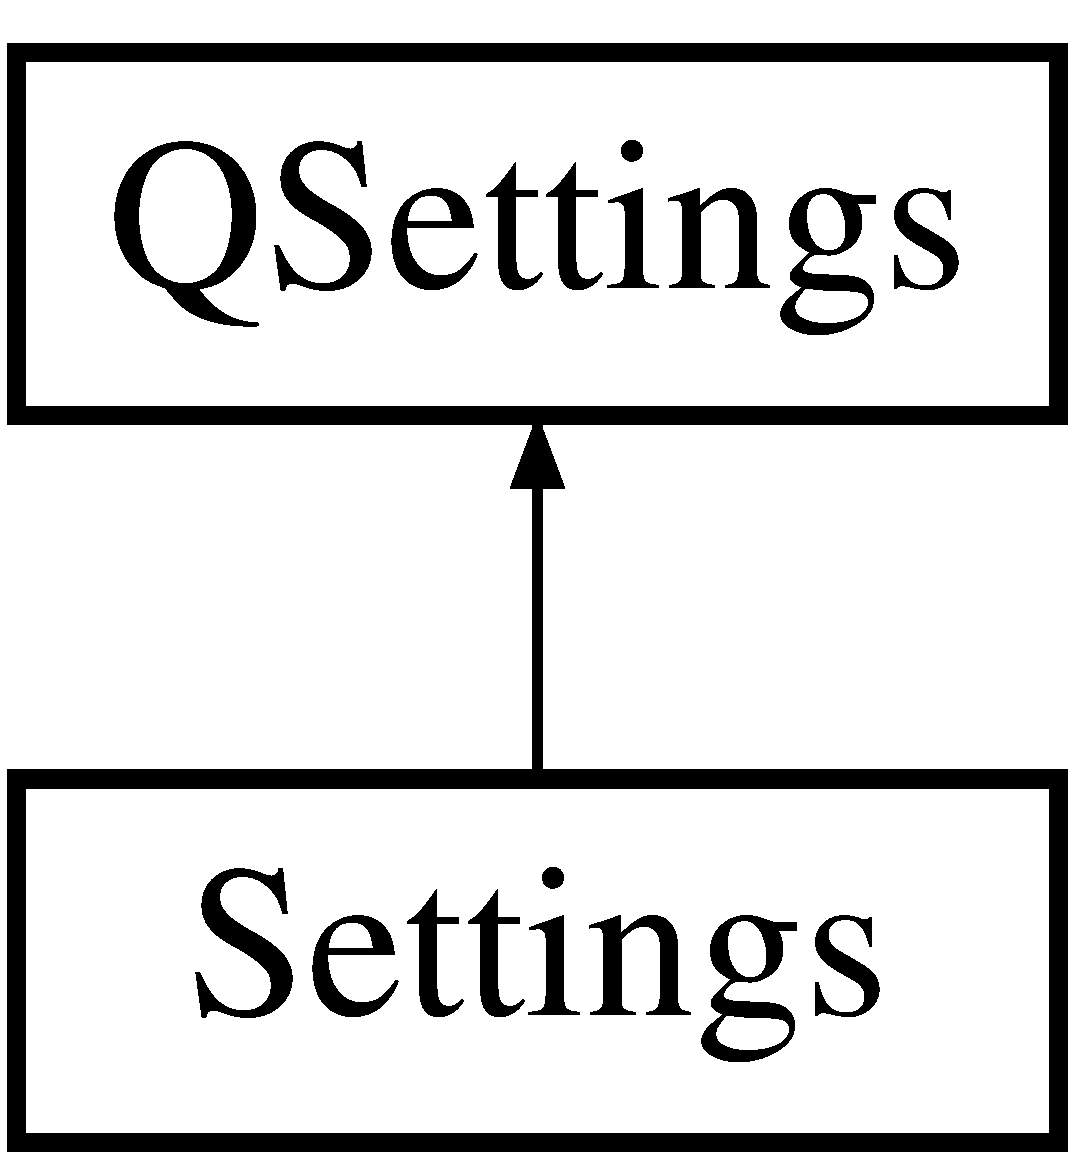
\includegraphics[height=2.000000cm]{class_settings}
\end{center}
\end{figure}
\subsection*{Public Member Functions}
\begin{DoxyCompactItemize}
\item 
\mbox{\Hypertarget{class_settings_ab7169a6eefce79566dd07db3b1e5e967}\label{class_settings_ab7169a6eefce79566dd07db3b1e5e967}} 
\hyperlink{class_settings_ab7169a6eefce79566dd07db3b1e5e967}{Settings} ()
\begin{DoxyCompactList}\small\item\em \hyperlink{class_settings}{Settings} Default constructor to create and initialise application settings. \end{DoxyCompactList}\end{DoxyCompactItemize}
\subsection*{Static Public Attributes}
\begin{DoxyCompactItemize}
\item 
\mbox{\Hypertarget{class_settings_af6945ac592f223dfedb6e4fdeced2ad9}\label{class_settings_af6945ac592f223dfedb6e4fdeced2ad9}} 
static Q\+String {\bfseries Main\+Window\+Geometry\+Key} = \char`\"{}Main\+Window\+Geometry\char`\"{}
\item 
\mbox{\Hypertarget{class_settings_a175ef5f25c13923b7b3ddfff3bb4221e}\label{class_settings_a175ef5f25c13923b7b3ddfff3bb4221e}} 
static Q\+String {\bfseries Logging\+Level\+Key} = \char`\"{}Logging\+Level\char`\"{}
\item 
\mbox{\Hypertarget{class_settings_ae1c484d451e8675ea3dc27ec3292a7d0}\label{class_settings_ae1c484d451e8675ea3dc27ec3292a7d0}} 
static Q\+String {\bfseries Overwrite\+Files\+Key} = \char`\"{}Overwrite\+Files\char`\"{}
\item 
\mbox{\Hypertarget{class_settings_a0a2907802c0b58e529d7e3b5b37616e2}\label{class_settings_a0a2907802c0b58e529d7e3b5b37616e2}} 
static Q\+String {\bfseries Input\+Dir\+Key} = \char`\"{}Input\+Dir\char`\"{}
\item 
\mbox{\Hypertarget{class_settings_a5a587a8a4ea1391953b5cfd8e9cc8924}\label{class_settings_a5a587a8a4ea1391953b5cfd8e9cc8924}} 
static Q\+String {\bfseries Output\+Dir\+Key} = \char`\"{}Output\+Dir\char`\"{}
\item 
\mbox{\Hypertarget{class_settings_a4b8f9b74462fd344f6807927d655ff63}\label{class_settings_a4b8f9b74462fd344f6807927d655ff63}} 
static Q\+String {\bfseries Patient\+Name\+Key} = \char`\"{}Patient\+Name\char`\"{}
\item 
\mbox{\Hypertarget{class_settings_ab97c9e2185f216041271820d6623f024}\label{class_settings_ab97c9e2185f216041271820d6623f024}} 
static Q\+String {\bfseries Patient\+I\+D\+Key} = \char`\"{}Patient\+ID\char`\"{}
\item 
\mbox{\Hypertarget{class_settings_a440dffe06be1b6ee9d93d040147622df}\label{class_settings_a440dffe06be1b6ee9d93d040147622df}} 
static Q\+String {\bfseries Patient\+D\+O\+B\+Key} = \char`\"{}Patient\+D\+OB\char`\"{}
\item 
\mbox{\Hypertarget{class_settings_a3aa6f82ed9e19607325b2b840aa45514}\label{class_settings_a3aa6f82ed9e19607325b2b840aa45514}} 
static Q\+String {\bfseries Patient\+Sex\+Key} = \char`\"{}Patient\+Sex\char`\"{}
\item 
\mbox{\Hypertarget{class_settings_a000551ce2bc5b741e7910233a4a6fae6}\label{class_settings_a000551ce2bc5b741e7910233a4a6fae6}} 
static Q\+String {\bfseries Study\+Description\+Key} = \char`\"{}Study\+Description\char`\"{}
\item 
\mbox{\Hypertarget{class_settings_a5ab483f6086f888f699ca812e0b60ca9}\label{class_settings_a5ab483f6086f888f699ca812e0b60ca9}} 
static Q\+String {\bfseries Study\+I\+D\+Key} = \char`\"{}Study\+ID\char`\"{}
\item 
\mbox{\Hypertarget{class_settings_afa7f2cee01d025e612fd448fbc583986}\label{class_settings_afa7f2cee01d025e612fd448fbc583986}} 
static Q\+String {\bfseries Study\+Modality\+Key} = \char`\"{}Study\+Modality\char`\"{}
\item 
\mbox{\Hypertarget{class_settings_a3bb79fe2a421be94c6f845b8b8a0ce7a}\label{class_settings_a3bb79fe2a421be94c6f845b8b8a0ce7a}} 
static Q\+String {\bfseries Study\+Date\+Time\+Key} = \char`\"{}Study\+Date\+Time\char`\"{}
\item 
\mbox{\Hypertarget{class_settings_a5da5fb9d4aaaa84e6c56c5b63e36f283}\label{class_settings_a5da5fb9d4aaaa84e6c56c5b63e36f283}} 
static Q\+String {\bfseries Study\+Instance\+U\+I\+D\+Key} = \char`\"{}Study\+Study\+U\+ID\char`\"{}
\item 
\mbox{\Hypertarget{class_settings_a77972d6f417b106d7edc0f826cd4f0ce}\label{class_settings_a77972d6f417b106d7edc0f826cd4f0ce}} 
static Q\+String {\bfseries Series\+Description\+Key} = \char`\"{}Series\+Description\char`\"{}
\item 
\mbox{\Hypertarget{class_settings_a689eb61798d61f0e1bc4cee562d857f1}\label{class_settings_a689eb61798d61f0e1bc4cee562d857f1}} 
static Q\+String {\bfseries Series\+Number\+Key} = \char`\"{}Series\+Number\char`\"{}
\item 
\mbox{\Hypertarget{class_settings_a8a6a8089b66079cdebff184f6e66398a}\label{class_settings_a8a6a8089b66079cdebff184f6e66398a}} 
static Q\+String {\bfseries Series\+Patient\+Position\+Key} = \char`\"{}Series\+Patient\+Position\char`\"{}
\item 
\mbox{\Hypertarget{class_settings_af0e8f0337ae87adfaceaac445f82d4fd}\label{class_settings_af0e8f0337ae87adfaceaac445f82d4fd}} 
static Q\+String {\bfseries Series\+Time\+Increment\+Key} = \char`\"{}Time\+Increment\char`\"{}
\end{DoxyCompactItemize}


\subsection{Detailed Description}
The \hyperlink{class_settings}{Settings} class Class which saves and restores settings between executions. 

The static xxx\+Key members are keys used to look up the appropriate values. 

The documentation for this class was generated from the following files\+:\begin{DoxyCompactItemize}
\item 
settings.\+h\item 
settings.\+cpp\end{DoxyCompactItemize}

%--- End generated contents ---

% Index
\backmatter
\newpage
\phantomsection
\clearemptydoublepage
\addcontentsline{toc}{chapter}{Index}
\printindex

\end{document}
